% This LaTeX document needs to be compiled with XeLaTeX.
\documentclass[a4paper]{article}
\usepackage[utf8]{inputenc}
\usepackage{graphicx}
\usepackage[export]{adjustbox}
\graphicspath{{./images/}{../cose da aggiungere/pittogrammi/}{../cose da aggiungere/privacy_conformita/}}
\usepackage{amsmath}
\usepackage{amsfonts}
\usepackage{amssymb}
\usepackage[version=4]{mhchem}
\usepackage{stmaryrd}
\usepackage{caption}
\usepackage[fallback]{xeCJK}
\usepackage{polyglossia}
\usepackage{fontspec}

\usepackage{array}
\usepackage{tabularx}
\usepackage{float}
\usepackage{fontawesome5} 
\usepackage{tikz}  

\usepackage{newunicodechar}
%\IfFontExistsTF{Noto Serif CJK TC}
%{\setCJKmainfont{Noto Serif CJK TC}}
%{\IfFontExistsTF{STSong}
%  {\setCJKmainfont{STSong}}
%  {\IfFontExistsTF{Droid Sans Fallback}
%    {\setCJKmainfont{Droid Sans Fallback}}
%    {\setCJKmainfont{SimSun}}
%}}
%
\setmainlanguage{italian}
%\IfFontExistsTF{CMU Serif}
%{\setmainfont{CMU Serif}}
%{\IfFontExistsTF{DejaVu Sans}
%  {\setmainfont{DejaVu Sans}}
%  {\setmainfont{Georgia}}
%}
%
%\newunicodechar{□}{\ifmmode\square\else{$\square$}\fi}

\usepackage{titling}
\pretitle{\begin{center}
\includegraphics[width=\textwidth]{../cose da aggiungere/header_WATT+.png}\\[6em]}
	\posttitle{\end{center}}  

\title{\Huge{DRENALINPHA+}}
\date{}

\begin{document}
	
\maketitle
\begin{figure}[H]
	\centering
	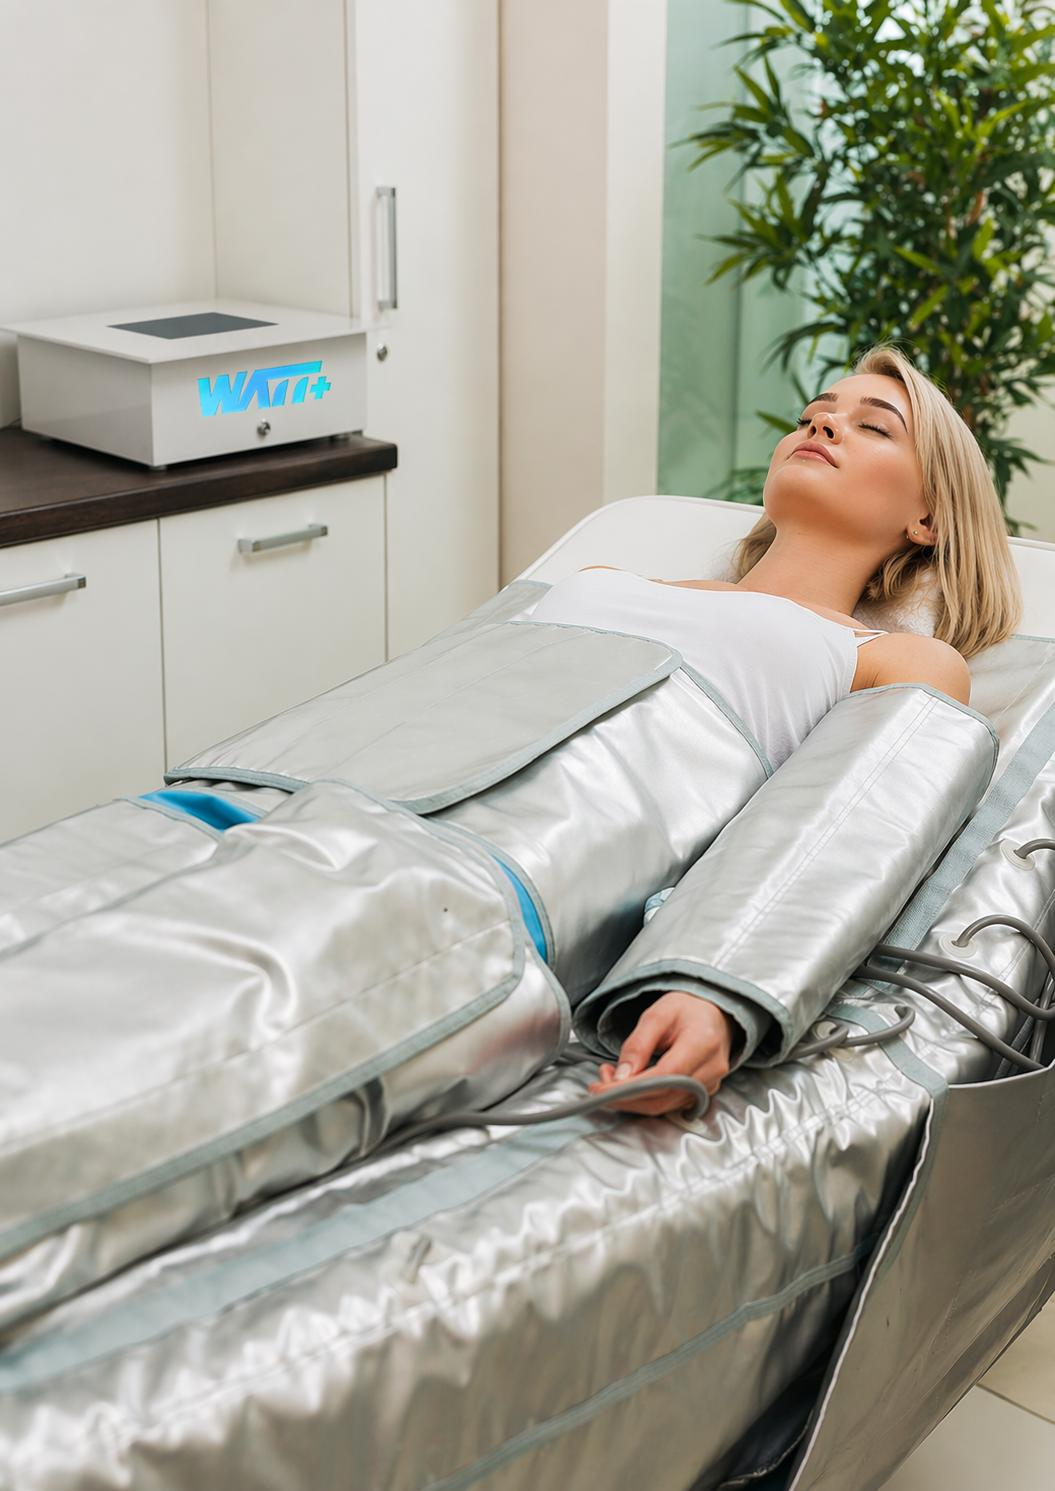
\includegraphics[width=0.6\linewidth]{images/DRENALINPHA+_copertina}
\end{figure}


\newpage

\noindent \faExclamationTriangle \textbf{CAUTION}:
\\
Tutte le persone che utilizzeranno l'Apparecchiatura devono studiare questo manuale con molta attenzione e, in seguito, prendere le misure di sicurezza necessarie, prima di iniziare una qualsiasi delle procedure. L'utilizzo errato di tale apparecchiatura potrebbe causare gravi danni alla salute del paziente/cliente.\\
II costruttore ed importatore possono variare le caratteristiche tecniche e le immagini senza alcun preavviso, potete contattarci per spiegazione e chiarimenti, le immagini utilizzate per il manuale sono solo indicative.

Si consiglia periodicamente di richiedere eventuali aggiornamenti del manuale e dei protocolli di lavoro. Tenersi periodicamente informati sulle normative vigenti.

Il trattamento deve essere eseguito solo ed esclusivamente da personale abilitato ed in ambienti idonei ed in regola con le vigenti norme nazionali e del territorio ove l'apparecchiatura viene installata.

Il presente manuale contiene dati e istruzioni generali per I'utilizzo e la manutenzione dell'apparecchiatura.\\
Il manuale per svolgere la sua funzione deve essere sempre a disposizione degli operatori e conservato per l'intera vita dell'apparecchiatura.\\
Il presente manuale costituisce parte integrante della macchina e deve perciò seguire il suo ciclo di vita, anche nel caso di trasferimento della stessa ad altro utilizzatore.\\
Per ogni qualsivoglia comunicazione inerente all'apparecchiatura, Vi preghiamo di citare sempre il numero di matricola riportato sul presente manuale e sulla targhetta a bordo macchina.\\
\textbf{Tutte le apparecchiature vengono sottoposte a collaudo prima della spedizione.}

\begin{itemize}
  \item \textbf{È responsabilità civile e penale di chi detiene o utilizza l'apparecchiatura seguire le indicazioni e le normative vigenti a livello nazionale o regionale ove l'apparecchiatura viene installata.}
  \item \textbf{È buona norma da parte dell'utilizzatore o acquirente verificare che l'apparecchiatura rientri nelle normative in vigore nel momento dell'acquisto.}
  \item \textbf{È buona norma che chi detiene la responsabilità all'interno di un istituto, studio, ambulatorio si mantenga aggiornato sulle normative in vigore e sui loro aggiornamenti.}
  \item \textbf{II trattamento deve essere eseguito solo ed esclusivamente da personale abilitato ed in ambienti idonei ed in regola con le vigenti norme nazionali e del territorio ove l'apparecchiatura viene installata.}
  \item \textbf{È vietato qualsiasi utilizzo dell'apparecchiatura in modo diverso da quanto espressamente previsto da questo manuale.}
  \item \textbf{All'interno degli ambienti di utilizzo devono essere osservate tutte le normative che regolamentano la sicurezza sul lavoro del personale e le normative che regolamentano la sicurezza degli ambienti.}
\end{itemize}
\textbf{La declina ogni responsabilità civile e penale per l'uso improprio dell'apparecchiatura.} All'interno sono stati inseriti volutamente degli errori grammaticali per scoraggiare l'uso improprio del presente manuale. Questi errori non vanno a inficiare la validità stessa del manuale, in quanto sono errori grammaticali o di forma.\\

\newpage

\tableofcontents

\newpage

\section{Ringraziamenti}
Vi ringraziamo per la preferenza accordataci, certi che troverete in questa apparecchiatura un valido contributo alla Vostra attività professionale; quest‘apparecchiatura utilizza la migliore e più moderna tecnologia per lo scopo cui esso è destinato.\\
Nel ringraziare i propri collaboratori, che hanno contribuito allo sviluppo di questo progetto, estende la sua gratitudine alla propria clientela per la fiducia e la disponibilità accordata.\\
Lo sviluppo e la costante ricerca, a garanzia di una sempre migliore efficienza delle apparecchiature, diventa così occasione per confrontarsi\\
ed arricchire le reciproche esperienze a tutto vantaggio di una clientela sempre più esigente e selettiva.

\vspace{10pt}
Troverai il marchio CE sulla Dichiarazione di Conformità.

\vspace{10pt}
\textbf{L'IMPORTANZA PER IL CLIENTE CHE ACQUISTA UN'APPARECCHIATURA È DI SAPERE CHE IL PROPRIO FORNITORE È ISCRITTO AL REGISTRO AEE. QUESTO COMPORTA CHE A FINE VITA DELL'APPARECCHIATURA IL CLIENTE NON DOVRA' SOSTENERE IN PROPRIO LE INGENTI SPESE PER LO SMALTIMENTO DEL BENE, MA SI POTRA' RIVOLGERE AL PROPRIO FORNITORE O AZIENDA AUTORIZZATA.}

\subsection{Informazione sul Manuale d'Uso}

\begin{center}
	
\includegraphics[max width=\textwidth, alt={}]{88087b73-f534-48df-a915-fe697c64a27c-06_107_120_741_221}
\end{center}

Per la sicurezza dei vostri trattamenti e la protezione del sistema, si prega di leggere il manuale prima di utilizzare l'apparecchiatura e di conservarlo con cura.\\
Questo Manuale fornisce informazioni per la messa in opera ed il corretto utilizzo dell'apparecchio.\\
È una guida di riferimento indispensabile per l'utente: \textbf{prima di installare e utilizzare la macchina è FONDAMENTALE leggere attentamente il contenuto del manuale e tenerlo sempre a portata di mano per una rapida consultazione}.

\textbf{L'inosservanza, anche parziale, delle raccomandazioni in esso contenute può dar luogo, oltre a malfunzionamenti, anche a danni all'apparecchiatura con invalidazione della garanzia.}

Solo seguendo scrupolosamente le prescrizioni e le raccomandazioni fornite dal costruttore si ha la certezza si ottenere i massimi risultati e di usufruire, in caso di necessità, di un servizio di assistenza tecnica veloce ed efficiente.

Il contenuto del presente manuale può subire delle variazioni senza preavviso, tali ragioni possono essere di ragione commerciale o tecnica, il manuale è solo a scopo divulgativo.

Il manuale è puramente tecnico, eventuali informazioni riportate sul modo di utilizzo della macchina sono puramente indicative.

Il trattamento deve essere eseguito solo ed esclusivamente da personale abilitato ed in ambienti idonei ed in regola con le vigenti norme nazionali e del territorio ove l'apparecchiatura viene installata.

La formazione del personale addetto all'uso dell'apparecchiatura è a carico del cliente / acquirente. In caso di dubbi sul trattamento chiedere sempre consiglio al costruttore / distributore ed in alcuni casi a personale abilitato\\
Leggere le istruzioni prima di procedere all'utilizzo della macchina Nel caso di malfunzionamenti non risolvibili da parte dell'utente rivolgersi al servizio di assistenza tecnica\\
\textbf{Non usare questa Apparecchiatura per problematiche o patologie di natura medica}

\subsection{Attenzione}
Solo il personale autorizzato e che ne possiede i requisiti può effettuare la manutenzione ordinaria e straordinaria di questa macchina. Qualsiasi manomissione o riparazione effettuata da personale non autorizzato e/o privo dei requisiti tecnici, e l'utilizzo di pezzi di ricambio non originali, fa decadere la garanzia e la responsabilità del prodotto da parte del costruttore / importatore.\\
Questo manuale descrive le istruzioni per utilizzare la macchina in sicurezza, leggerlo molto attentamente per comprendere appieno il funzionamento e la manutenzione della macchina, prima di iniziare qualsiasi procedura.\\
\textbf{Tutte le persone che utilizzeranno l'apparecchiatura devono studiare questo manuale con molta attenzione ed in seguito, prendere le misure di sicurezza necessarie prima di iniziare una qualsiasi delle procedure.}\\
La formazione del personale addetto all'uso dell'apparecchiatura è a carico del cliente / acquirente.\\
Non aprire la macchina o effettuare manutenzioni, tali operazioni sono delegate esclusivamente a personale autorizzato.\\
Leggere le istruzioni prima di procedere all'utilizzo della macchina. Nel caso di malfunzionamenti non risolvibili da parte dell'utente rivolgersi al servizio di assistenza tecnica (vedi numero indicato nella copertina)

La formazione del personale addetto all'uso dell'apparecchiatura è a carico del cliente/acquirente.\\
Non aprire la macchina o effettuare manutenzioni, tali operazioni sono delegate esclusivamente al personale autorizzato.\\
Leggere le istruzioni prima di procedere all'utilizzo della macchina. Nel caso di malfunzionamenti non risolvibili da parte dell'utente rivolgersi al servizio di assistenza tecnica (vedi numero indicato nella copertina)

\noindent \faExclamationTriangle \textbf{CAUTION}:
\\
\textbf{\textit{Tutte le persone che utilizzeranno la macchina devono studiare questo manuale con molta attenzione e, in seguito, prendere le misure di sicurezza necessarie, prima di iniziare una qualsiasi delle procedure. L'utilizzo errato di tale apparecchiatura potrebbe causare gravi danni alla salute}}

\subsection{Simboli}

\begin{figure}[H]
	\centering
	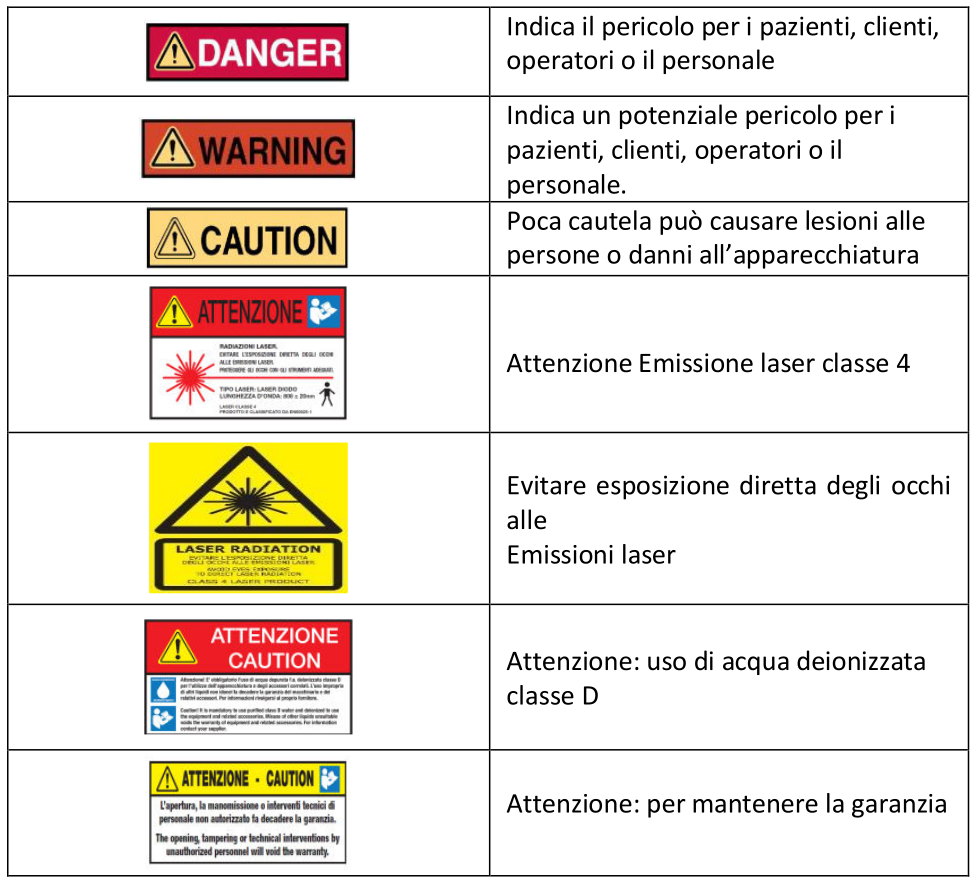
\includegraphics[width=\linewidth]{pittogrammi_1}
%	\caption{}
	\label{fig:pittogrammi1}
\end{figure}
\begin{figure}[H]
	\centering
	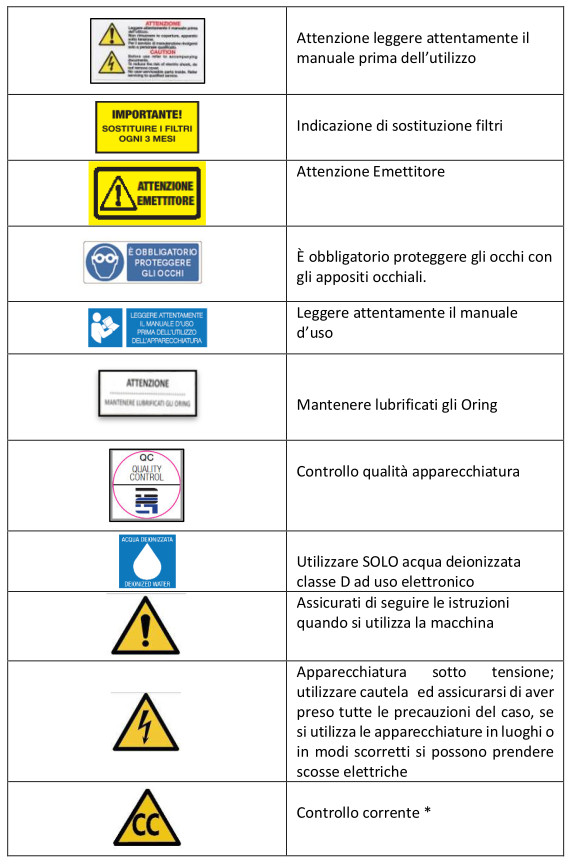
\includegraphics[width=\linewidth]{pittogrammi_2}
%	\caption{}
	\label{fig:pittogrammi2}
\end{figure}
\begin{figure}[H]
	\centering
	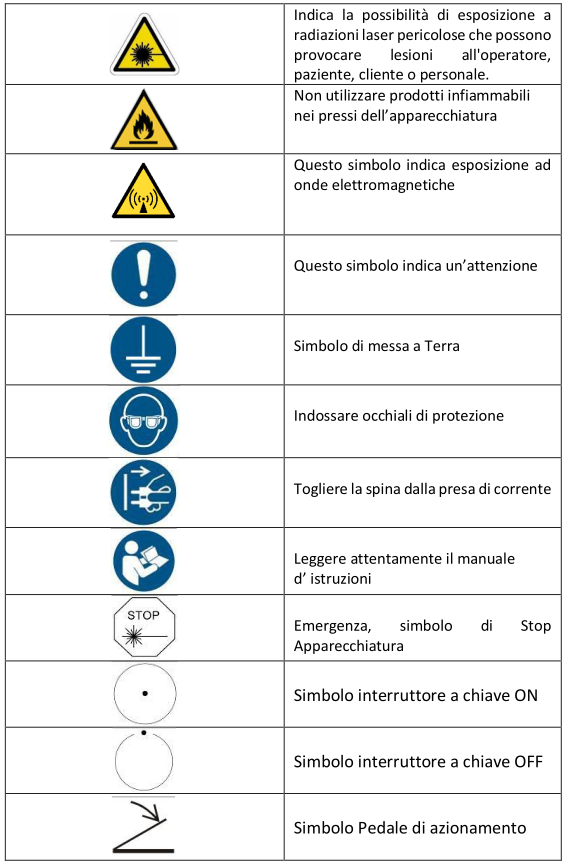
\includegraphics[width=\linewidth]{pittogrammi_3}
%	\caption{}
	\label{fig:pittogrammi3}
\end{figure}
\begin{figure}[H]
	\centering
	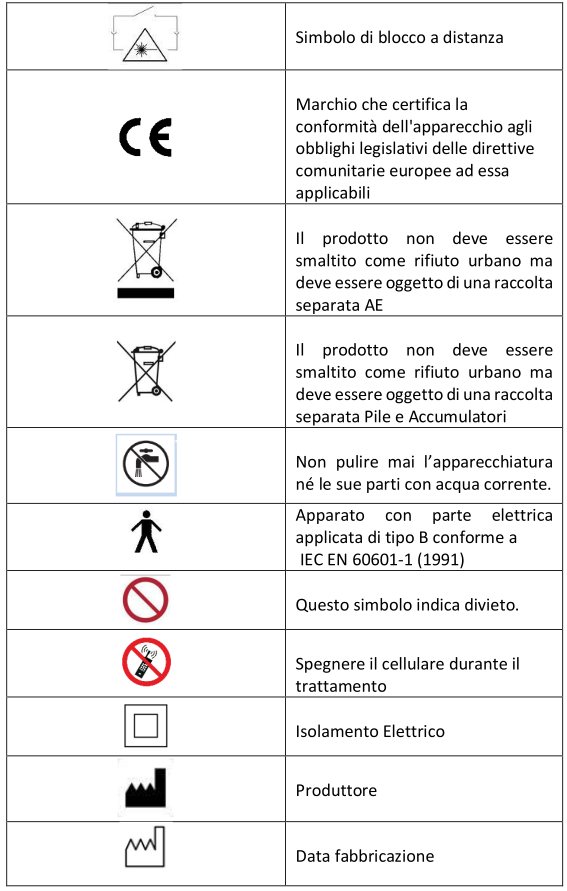
\includegraphics[width=\linewidth]{pittogrammi_4}
%	\caption{}
	\label{fig:pittogrammi4}
\end{figure}
\begin{figure}[H]
	\centering
	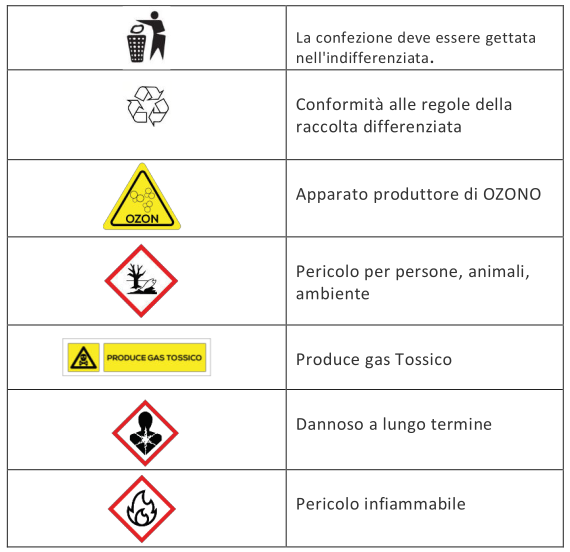
\includegraphics[width=\linewidth]{pittogrammi_5}
%	\caption{}
	\label{fig:pittogrammi5}
\end{figure}


%\section{SIMBOLI}
%\begin{center}
%\begin{tabularx}{\textwidth}{|X|X|}
%\hline
%\begin{tabular}{l}
%
\includegraphics[max width=\textwidth, alt={}]{88087b73-f534-48df-a915-fe697c64a27c-09_58_54_915_312}
% \\
%DANGER \\
%\end{tabular} & Indica il pericolo per i pazienti, clienti, operatori o il personale \\
%\hline
%\begin{tabular}{l}
%
\includegraphics[max width=\textwidth, alt={}]{88087b73-f534-48df-a915-fe697c64a27c-09_60_69_1020_303}
% \\
%WARNING \\
%\end{tabular} & Indica un potenziale pericolo per i pazienti, clienti, operatori o il personale. \\
%\hline
%\begin{tabular}{l}
%
\includegraphics[max width=\textwidth, alt={}]{88087b73-f534-48df-a915-fe697c64a27c-09_65_63_1118_307}
% \\
%CAUTION \\
%\end{tabular} & Poca cautela può causare lesioni alle persone o danni all'apparecchiatura \\
%\hline
%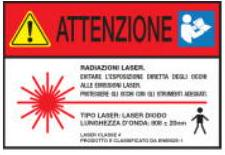
\includegraphics[max width=\textwidth, alt={}]{88087b73-f534-48df-a915-fe697c64a27c-09_155_225_1204_307}
% & Attenzione Emissione laser classe 4 \\
%\hline
%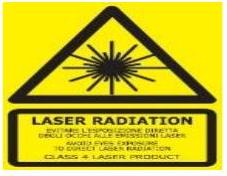
\includegraphics[max width=\textwidth, alt={}]{88087b73-f534-48df-a915-fe697c64a27c-09_176_227_1376_307}
% & \begin{tabular}{l}
%Evitare esposizione diretta degli occhi alle \\
%Emissioni laser \\
%\end{tabular} \\
%\hline
%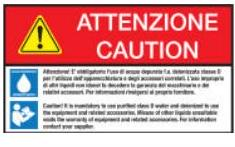
\includegraphics[max width=\textwidth, alt={}]{88087b73-f534-48df-a915-fe697c64a27c-09_147_235_1569_301}
% & Attenzione: uso di acqua deionizzata classe D \\
%\hline
%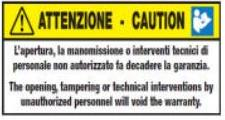
\includegraphics[max width=\textwidth, alt={}]{88087b73-f534-48df-a915-fe697c64a27c-09_120_225_1729_307}
% & Attenzione: per mantenere la garanzia \\
%\hline
%\end{tabularx}
%\end{center}
%
%Pag. 8\\
%Mod. Rev.1.0 SLV 09-2020
%
%\begin{center}
%\begin{tabular}{|l|l|}
%\hline
%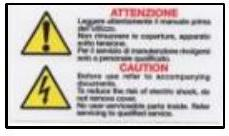
\includegraphics[max width=\textwidth, alt={}]{88087b73-f534-48df-a915-fe697c64a27c-10_136_229_152_379}
% & Attenzione leggere attentamente il manuale prima dell'utilizzo \\
%\hline
%\begin{tabular}{l}
%IMPORTANTE! \\
%SOSTITUIRE I FILTRI \\
%OGNI 3 MESI \\
%\end{tabular} & Indicazione di sostituzione filtri \\
%\hline
%
\includegraphics[max width=\textwidth, alt={}]{88087b73-f534-48df-a915-fe697c64a27c-10_120_228_429_379}
% & Attenzione Emettitore \\
%\hline
%
\includegraphics[max width=\textwidth, alt={}]{88087b73-f534-48df-a915-fe697c64a27c-10_94_239_575_366}
% & È obbligatorio proteggere gli occhi con gli appositi occhiali. \\
%\hline
%\begin{tabular}{l}
%
\includegraphics[max width=\textwidth, alt={}]{88087b73-f534-48df-a915-fe697c64a27c-10_82_72_704_378}
% \\
%LEGGERE ATTENTAMENTE \\
%IL MANUALE D'USO PRIMA DELUTIUZZO DELMAPSARECOHATURA \\
%\end{tabular} & Leggere attentamente il manuale d'uso \\
%\hline
%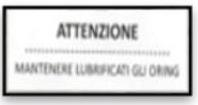
\includegraphics[max width=\textwidth, alt={}]{88087b73-f534-48df-a915-fe697c64a27c-10_105_198_821_397}
% & Mantenere lubrificati gli Oring \\
%\hline
%
\includegraphics[max width=\textwidth, alt={}]{88087b73-f534-48df-a915-fe697c64a27c-10_146_152_976_417}
% & Controllo qualità apparecchiatura \\
%\hline
%
\includegraphics[max width=\textwidth, alt={}]{88087b73-f534-48df-a915-fe697c64a27c-10_109_113_1140_440}
% & Utilizzare SOLO acqua deionizzata classe D ad uso elettronico \\
%\hline
%
\includegraphics[max width=\textwidth, alt={}]{88087b73-f534-48df-a915-fe697c64a27c-10_120_139_1256_420}
% & Assicurati di seguire le istruzioni quando si utilizza la macchina \\
%\hline
%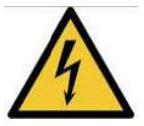
\includegraphics[max width=\textwidth, alt={}]{88087b73-f534-48df-a915-fe697c64a27c-10_126_144_1438_420}
% & Apparecchiatura sotto tensione; utilizzare cautela ed assicurarsi di aver preso tutte le precauzioni del caso, se si utilizza le apparecchiature in luoghi o in modi scorretti si possono prendere scosse elettriche \\
%\hline
%
\includegraphics[max width=\textwidth, alt={}]{88087b73-f534-48df-a915-fe697c64a27c-10_118_140_1624_423}
% & Controllo corrente * \\
%\hline
%\end{tabular}
%\end{center}
%
%\begin{center}
%\begin{tabular}{|l|l|}
%\hline
%
\includegraphics[max width=\textwidth, alt={}]{88087b73-f534-48df-a915-fe697c64a27c-11_124_136_148_353}
% & Indica la possibilità di esposizione a radiazioni laser pericolose che possono provocare lesioni all'operatore, paziente, cliente o personale. \\
%\hline
%
\includegraphics[max width=\textwidth, alt={}]{88087b73-f534-48df-a915-fe697c64a27c-11_127_139_289_350}
% & Non utilizzare prodotti infiammabili nei pressi dell’apparecchiatura \\
%\hline
%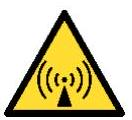
\includegraphics[max width=\textwidth, alt={}]{88087b73-f534-48df-a915-fe697c64a27c-11_120_132_427_353}
% & Questo simbolo indica esposizione ad onde elettromagnetiche \\
%\hline
%
\includegraphics[max width=\textwidth, alt={}]{88087b73-f534-48df-a915-fe697c64a27c-11_134_139_581_350}
% & Questo simbolo indica un'attenzione \\
%\hline
%
\includegraphics[max width=\textwidth, alt={}]{88087b73-f534-48df-a915-fe697c64a27c-11_131_137_732_350}
% & Simbolo di messa a Terra \\
%\hline
%
\includegraphics[max width=\textwidth, alt={}]{88087b73-f534-48df-a915-fe697c64a27c-11_130_139_868_350}
% & Indossare occhiali di protezione \\
%\hline
%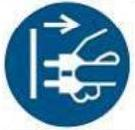
\includegraphics[max width=\textwidth, alt={}]{88087b73-f534-48df-a915-fe697c64a27c-11_130_135_1003_350}
% & Togliere la spina dalla presa di corrente \\
%\hline
%
\includegraphics[max width=\textwidth, alt={}]{88087b73-f534-48df-a915-fe697c64a27c-11_120_130_1138_355}
% & Leggere attentamente il manuale d' istruzioni \\
%\hline
%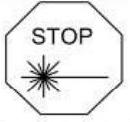
\includegraphics[max width=\textwidth, alt={}]{88087b73-f534-48df-a915-fe697c64a27c-11_122_130_1266_355}
% & Emergenza, simbolo di Stop Apparecchiatura \\
%\hline
%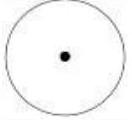
\includegraphics[max width=\textwidth, alt={}]{88087b73-f534-48df-a915-fe697c64a27c-11_120_132_1395_355}
% & Simbolo interruttore a chiave ON \\
%\hline
%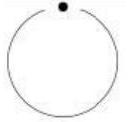
\includegraphics[max width=\textwidth, alt={}]{88087b73-f534-48df-a915-fe697c64a27c-11_122_128_1520_355}
% & Simbolo interruttore a chiave OFF \\
%\hline
%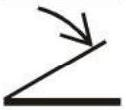
\includegraphics[max width=\textwidth, alt={}]{88087b73-f534-48df-a915-fe697c64a27c-11_110_126_1651_355}
% & Simbolo Pedale di azionamento \\
%\hline
%\end{tabular}
%\end{center}
%
%\begin{center}
%\begin{tabular}{|l|l|}
%\hline
%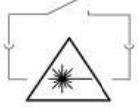
\includegraphics[max width=\textwidth, alt={}]{88087b73-f534-48df-a915-fe697c64a27c-12_107_139_144_422}
% & Simbolo di blocco a distanza \\
%\hline
%$C$ & Marchio che certifica la conformità dell'apparecchio agli obblighi legislativi delle direttive comunitarie europee ad essa applicabili \\
%\hline
%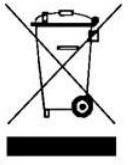
\includegraphics[max width=\textwidth, alt={}]{88087b73-f534-48df-a915-fe697c64a27c-12_165_128_542_431}
% & Il prodotto non deve essere smaltito come rifiuto urbano ma deve essere oggetto di una raccolta separata AE \\
%\hline
%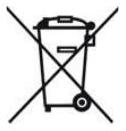
\includegraphics[max width=\textwidth, alt={}]{88087b73-f534-48df-a915-fe697c64a27c-12_131_126_773_431}
% & Il prodotto non deve essere smaltito come rifiuto urbano ma deve essere oggetto di una raccolta separata Pile e Accumulatori \\
%\hline
%
\includegraphics[max width=\textwidth, alt={}]{88087b73-f534-48df-a915-fe697c64a27c-12_126_126_954_431}
% & Non pulire mai l'apparecchiatura né le sue parti con acqua corrente. \\
%\hline
%穴 & Apparato con parte elettrica applicata di tipo B conforme a IEC EN 60601-1 (1991) \\
%\hline
%
\includegraphics[max width=\textwidth, alt={}]{88087b73-f534-48df-a915-fe697c64a27c-12_102_103_1220_441}
% & Questo simbolo indica divieto. \\
%\hline
%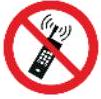
\includegraphics[max width=\textwidth, alt={}]{88087b73-f534-48df-a915-fe697c64a27c-12_99_101_1346_443}
% & Spegnere il cellulare durante il trattamento \\
%\hline
%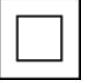
\includegraphics[max width=\textwidth, alt={}]{88087b73-f534-48df-a915-fe697c64a27c-12_83_87_1477_453}
% & Isolamento Elettrico \\
%\hline
%
\includegraphics[max width=\textwidth, alt={}]{88087b73-f534-48df-a915-fe697c64a27c-12_83_89_1592_447}
% & Produttore \\
%\hline
%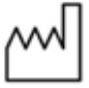
\includegraphics[max width=\textwidth, alt={}]{88087b73-f534-48df-a915-fe697c64a27c-12_88_89_1704_447}
% & Data fabbricazione \\
%\hline
%\end{tabular}
%\end{center}
%
%\begin{center}
%\begin{tabular}{|l|l|}
%\hline
%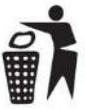
\includegraphics[max width=\textwidth, alt={}]{88087b73-f534-48df-a915-fe697c64a27c-13_109_85_138_379}
% & La confezione deve essere gettata nell'indifferenziata. \\
%\hline
%
\includegraphics[max width=\textwidth, alt={}]{88087b73-f534-48df-a915-fe697c64a27c-13_89_93_281_375}
% & Conformità alle regole della raccolta differenziata \\
%\hline
%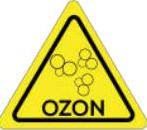
\includegraphics[max width=\textwidth, alt={}]{88087b73-f534-48df-a915-fe697c64a27c-13_130_147_433_338}
% & Apparato produttore di OZONO \\
%\hline
%
\includegraphics[max width=\textwidth, alt={}]{88087b73-f534-48df-a915-fe697c64a27c-13_148_151_585_334}
% & Pericolo per persone, animali, ambiente \\
%\hline
%\begin{tabular}{l}
%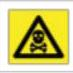
\includegraphics[max width=\textwidth, alt={}]{88087b73-f534-48df-a915-fe697c64a27c-13_73_73_769_260}
% \\
%PRODUCE GAS TOSSICO \\
%\end{tabular} & Produce gas Tossico \\
%\hline
%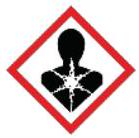
\includegraphics[max width=\textwidth, alt={}]{88087b73-f534-48df-a915-fe697c64a27c-13_138_139_880_346}
% & Dannoso a lungo termine \\
%\hline
%
\includegraphics[max width=\textwidth, alt={}]{88087b73-f534-48df-a915-fe697c64a27c-13_144_143_1024_338}
% & Pericolo infiammabile \\
%\hline
%\end{tabular}
%\end{center}

\subsection{Requisiti ambientali}
L'ambiente deve essere sempre sufficientemente areato e pulito, la polvere e altri agenti quali ad esempio il gel, possono danneggiare parti dell'apparecchiatura.\\
\textbf{Ad ogni fine trattamento pulire tutti i manipoli ed accessori}. Prestare attenzione alla pulizia del manipolo e disinfettare ogni parte che viene a contatto con i clienti.

Per garantire il miglior funzionamento possibile la temperatura interna dei locali deve essere mantenuta tra i $20^{\circ} \mathrm{C}$ e $25^{\circ} \mathrm{C}$, la relativa umidità consigliata per un perfetto utilizzo deve essere inferiore al $60 \%$. È consigliato mantenere la temperatura ambiente al di sotto dei 28 gradi, in caso di necessità intervenire con ausili quali: condizionatore o

Pag. 12\\
Mod. Rev.1.0 SLV 09-2020\\
ventilatore.\\
L'apparecchiatura deve essere tenuta lontano da fonti di calore (caloriferi) e deve essere tenuta ad una distanza di oltre 60 cm da altri oggetti. Ciò permette di evitare interferenze e collisioni.

\subsection{Disimballaggio}
Estrarre la macchina con cura dalla scatola e posizionarla nel luogo prestabilito e adatto.\\
Verificare l'integrità dell'apparecchiatura e degli accessori.\\
\textbf{Smaltire in modo corretto gli imballi.}

\subsection{Garanzia}
Tutti gli articoli, ove previsto, sono coperti da garanzia di legge da parte del costruttore e/o distributore\\
Fa fede la data di acquisto riportata in fattura.\\
Nel caso di acquisto da un nostro rivenditore/distributore, fa fede la data di acquisto del Rivenditore.

\begin{itemize}
  \item 24 Mesi per articoli destinati ad uso non professionale
  \item 12 Mesi per articoli venduti con Partita Iva e per uso professionale Non sono coperte da garanzia tutte le parti soggette ad usura o usate in modo improprio ed errato.\\
Sono escluse dalla garanzia rotture causate da caduta o negligenza da parte del cliente.\\
Le riparazioni saranno effettuate presso i centri assistenza autorizzati, o presso la nostra sede, saranno a carico del cliente la spesa di trasporto e spedizione (Franco fabbrica).\\
In caso di intervento presso la sede del cliente dovrà essere riconosciuta al servizio di assistenza il diritto di chiamata (vedere listino). Il diritto di chiamata non è dovuto entro il primo mese dopo l'acquisto) Nel periodo di garanzia verranno addebitati ai clienti quella tipologia di interventi tecnici ritenuti a VUOTO, se durante un intervento non si dovessero riscontrare anomalie o malfunzionamenti dovuti a negligenza e mancata manutenzione ordinaria, oppure ad una cattiva preparazione dell'operatore.\\
\subsubsection{La garanzia decade nei seguenti casi:}
  \item Se l'apparecchiatura non ha avuto la dovuta manutenzione periodica e nel caso essa venga aperta da personale non autorizzato.
  \item Collocazione, installazione e messa in opera non adeguata;
  \item Utilizzo scorretto o non conforme alle prescrizioni di questo manuale;
  \item Manutenzione impropria o inadeguata da parte dell'utente;
  \item Funzionamento non conforme alle specifiche ambientali indicate per il prodotto;
  \item Apertura non autorizzata degli involucri esterni;
  \item Manomissioni e/o modifiche non autorizzate;
  \item Utilizzo di accessori non originali.
  \item Danni causati da corpi estranei, acqua, agenti chimici, terra, sabbia, trucioli metallici, sostanze organiche, ecc.
  \item La garanzia è valida dalla data di acquisto dell'apparecchiatura, per garanzia si intende solo ed esclusivamente la riparazione gratuita e la sostituzione delle parti che risultino difettose dall'origine.
\end{itemize}

Eventuali fermi apparecchiatura non danno adito a prolungamenti della garanzia e /o rimborsi per fermo macchina e quant' altro.\\
garantisce la qualità dei propri apparecchi, \textbf{quando utilizzati in accordo con le istruzioni fornite in questo manuale.}

\vspace{10pt}
\noindent \faExclamationTriangle \textbf{CAUTION:} 
\\
\textbf{\textit{Tutte le persone che utilizzeranno la macchina devono studiare questo manuale con molta attenzione e, in seguito, prendere le misure di sicurezza necessarie, prima di iniziare una qualsiasi delle procedure. L'utilizzo errato di tale apparecchiatura potrebbe causare gravi danni alla salute del cliente/paziente. La mancata manutenzione periodica e l'utilizzo di pezzi di ricambio non originali fa perdere i diritti di garanzia e la responsabilità di prodotto.}}

\subsection{Servizio Assistenza}
La nostra azienda offre un perfetto servizio di vendita e servizio di postvendita tra cui l'installazione, la formazione e la manutenzione. Tutti i prodotti hanno, per uso professionale, un anno di garanzia.\\
La consulenza tecnica e gli aggiornamenti del software sono a pagamento.

\subsection{\faCopyright[regular] Copyright}
I contenuti di questo manuale - grafica, testi, tabelle, immagini, e ogni altra informazione disponibile e in qualunque forma sono riservati. Salvo espressamente autorizzato, è vietata la divulgazione e duplicazione del contenuto di tale manuale; qualsiasi violazione implicherà l'obbligo di risarcimento dei danni. Tutti i diritti sono riservati.

\subsection{Tutela e riservatezza dei dati}
Il venditore comunica che i dati personali, forniti nella procedura di ordine (telematico o telefonico), formano oggetto di trattamento ai sensi del regolamento europeo UE sul trattamento dei dati personali (GDPR). Tali dati rimangono a disposizione del consumatore per la verifica, modificazione o cancellazione e per l'esercizio di ogni altro diritto previsto. La raccolta ed il trattamento dei dati del consumatore sono necessari nel caso in cui volesse fare un ordine di prodotti o per accedere a particolari servizi di fidelizzazione. I dati del consumatore potranno essere comunicati dallo staff del venditore o comunicati a terzi non dipendenti necessari o funzionali per lo svolgimento dell'attività contrattuale (Istituti bancari per la gestione dei pagamenti e spedizionieri per il trasporto).

\textbf{Il contenuto del presente manuale può subire delle variazioni senza preavviso, tali ragioni possono essere di ragione commerciale o tecnica, il manuale è solo a scopo divulgativo}. Il manuale è puramente tecnico, eventuali informazioni riportate sul modo di utilizzo della macchina sono puramente indicative, per il trattamento esso deve essere eseguito solo ed esclusivamente da personale abilitato ed in ambienti idonei ed in regola.

\subsection{Smaltimento}
L'apparecchiatura come tutte le apparecchiature elettroniche e composte da materiali plastici deve essere smaltita secondo la normativa 2002/96/CE del consiglio europeo per lo smaltimento dei rifiuti.\\
La direttiva RAEE si pone l'obiettivo di diminuire il volume dei rifiuti derivanti da apparecchiature elettriche ed elettroniche a fine vita, riducendo contemporaneamente l'immissione nell'ambiente delle sostanze pericolose vietate dalla direttiva ROHS.

La normativa prevede che a fine vita alcune apparecchiature elettriche ed elettroniche non possano essere conferite in discarica ma debbano essere gestite da un sistema che preveda la loro raccolta separata e uno specifico trattamento di reimpiego, riciclaggio o altre forme di recupero per prodotti finiti, componenti e materiali. In questa ottica, la direttiva 2002/96/CE incoraggia le aziende a promuovere modifiche in sede di progettazione dei prodotti che rendano le apparecchiature più semplici da smaltire, recuperare e riciclare.

\textbf{Richiedere eventuali informazioni al servizio di assistenza.}

\subsection{Foro competente}
Per ogni controversia, sarà competente in via esclusiva il Foro di Bergamo.

\section{Sicurezza e funzionalità}
\noindent \faExclamationTriangle \textbf{CAUTION:}
\\
Tutte le persone che utilizzeranno la macchina devono studiare questo manuale con molta attenzione ed in seguito, prendere le misure di sicurezza necessarie, prima di iniziare una qualsiasi delle procedure. L'utilizzo errato di tale apparecchiatura potrebbe causare gravi danni alla salute del cliente.

\subsection{Funzionalità e sicurezza}
L'apparecchiatura è conforme alle direttive europee sulla sicurezza degli apparecchi elettrici: vedere \textbf{Dichiarazione di conformità} alla fine del manuale.\\
L'utilizzatore viene informato dei rischi che l'utilizzo delle apparecchiature ad alta tecnologia possono comportare es. elettrici, incendio e biologici e si assume la responsabilità di operare in base alle leggi vigenti nel paese d'utilizzo e di operare in piena sicurezza osservando le indicazioni del manuale d'uso, tenendo inoltre presente le regole dell'istituto dettate dalle norme sulla sicurezza interna, norme antincendio e norme sulla prevenzione degli incidenti sul lavoro.

\vspace{10pt}
\noindent \textbf{È responsabilità di chi detiene la titolarità dell'attività di estetista:}
\begin{itemize}
  \item mantenere controlli di sicurezza
  \item fornire addestramento ad eventuale altro personale che utilizza (e collabora all'utilizzo) l'apparecchiatura
  \item fornire informazioni a coloro che ricevono il trattamento estetico e ad ogni altro visitatore.
\end{itemize}

\subsection{Rischi elettrici}
\begin{itemize}
  \item Il terminale di terra è contrassegnato in conformità con la norma pertinente, il personale della manutenzione dell'impianto elettrico dovrebbero controllare se la connessione sia consona alle esigenze.
  \item L'apparecchio è fornito di protezione di messa a terra tramite il cavo di alimentazione. Verificarne periodicamente la sua integrità.
  \item Il distributore o importatore non è responsabile delle parti elettriche esterne all'apparecchiatura
  \item Solo il personale autorizzato può eseguire interventi tecnici
  \item Tenere tutti i pannelli di copertura dell'apparecchiatura chiusi. La rimozione delle coperture crea un pericolo\\
per la sicurezza elettrica e meccanica, solo personale autorizzato può eseguire tali operazioni
  \item Non lasciare mai l'apparecchio acceso, aperto o incustodito durante la manutenzione del sistema.
  \item Non utilizzare l'apparecchio se il cavo di alimentazione è danneggiato.
  \item Non bagnare o spruzzare l'apparecchiatura per la pulizia, eseguire sempre la pulizia dell'apparecchiatura con presa di corrente scollegata.
  \item Pulire il touch-screen solo a macchina spenta, l'utilizzo di prodotti non idonei può provocare danni e malfunzionamenti.
\end{itemize}

\subsection{Rischi incendio}
Mantenere qualsiasi materiale infiammabile lontano dall'apparecchiatura:

\begin{itemize}
  \item Fare attenzione a liquidi infiammabili nelle vicinanze esempio alcol, essi non devono venire a contatto con l'apparecchiatura.
  \item Fonti di ossigeno, quali bombole e generatori, se vengono a contatto con l'apparecchiatura si possono infiammare.
  \item Utilizzare l'apparecchiatura lontano da arredi infiammabili quali tende o stoffe
  \item Non utilizzare l'apparecchiatura con coperture che ne possano impedire la corretta ventilazione
  \item La stanza dove si utilizza la pressoterapia o l'istituto deve essere dotato di estintore
  \item Tenere oggetti infiammabili lontano dall'apparecchiatura
  \item Non utilizzare l'apparecchiatura in presenza di liquidi infiammabili (come alcool o acetone), gas infiammabili (come etere) o gas ossidanti, quali protossido di azoto (N2O) e di ossigeno.
\end{itemize}

\subsection{Sistemi di sicurezza}
L'apparecchiatura deve essere sottoposta a controlli periodici, per la sicurezza delle persone e per il suo corretto funzionamento.

Il produttore / importatore/ rivenditore garantiscono la sicurezza solo nel caso in cui:

\begin{itemize}
  \item L'apparecchiatura viene utilizzata solo in ambienti e da personale che ne abbia i requisiti
  \item L'apparecchiatura viene usata solo da personale formato.
  \item Gli utilizzatori abbiano preso atto delle istruzioni descritte sul manuale.
  \item Che gli impianti elettrici e di sicurezza siano in regola con le vigenti normative del paese di installazione.
  \item Che l'installazione, la manutenzione periodica e straordinaria sia stata eseguita correttamente e da personale autorizzato.
\end{itemize}

\subsection{Avvertenze}
\begin{itemize}
  \item Non utilizzare apparati cellulari durante ed in prossimità dell'apparecchiatura.
  \item Non utilizzare apparati ossigeno in prossimità dell'apparecchiatura.
  \item Non utilizzare l'apparecchiatura in prossimità di apparati di radiofrequenza.
  \item Tutto il personale deve prestare la massima attenzione e deve usare i sistemi di sicurezza durante l'uso dell'apparecchiatura
  \item L'apparecchiatura richiede la massima cura durante e dopo I'utilizzo.
  \item Solo persone che hanno ricevuto un adeguato training sull'apparecchiatura, prendendo in considerazione le istruzioni operative ed i rischi possibili, possono usare l'apparecchiatura.
  \item Operatori non qualificati e non istruiti non hanno il permesso di utilizzare l'apparecchiatura su sé stessi e su terzi.
  \item Ogni operatore deve aver letto e capito il manuale d'uso prima di dar inizio ai trattamenti.
  \item La sicurezza dei clienti dipende soprattutto dalla competenza che gli operatori, che utilizzano tale apparecchiatura, hanno acquisito grazie, anche, alla lettura\\
del presente manuale, oltre alle conoscenze e competenze acquisite tramite corsi esterni o similari.
  \item Gli operatori devono informare i clienti dei rischi che comporta l'uso della macchina.
  \item Il Processo del trattamento deve essere spiegato al cliente. Il cliente deve dare un consenso scritto al trattamento
  \item Illustrare al cliente le funzioni dell'apparecchio e le sensazioni percepite durante il trattamento
\end{itemize}

\textbf{Al termine di ogni trattamento pulire e disinfettare il kit con appositi prodotti e lasciare raffreddare le dotazioni aperte, in modo da evitare problemi di surriscaldamento ai circuiti interni. L'eventuale malfunzionamento derivante dal non rispetto di tale avvertenza, non verrà riconosciuto dal distributore/costruttore come danno in garanzia.}

\section{Sistema di funzionamento}
\noindent \faExclamationTriangle \textbf{CAUTION}:
\\
\textbf{Tutte le persone che utilizzeranno la macchina devono studiare questo manuale con molta attenzione ed in seguito, prendere le misure di sicurezza necessarie, prima di iniziare una qualsiasi delle procedure. L'utilizzo errato di tale apparecchiatura potrebbe causare gravi danni alla salute del cliente.}

\vspace{10pt}
L'apparecchio è azionato da un'elettropompa che immette aria in cuscinetti di varie forme e dimensioni che, a loro volta, vengono applicati, liberi o inseriti, in appositi contenitori di tessuto, plastica o altro materiale idoneo.\\
La regolazione della pressione di massaggio viene effettuata con appositi dispositivi e controllata da uno strumento di misura e da un dispositivo di sicurezza.\\
L'apparecchio è dotato inoltre, di dispositivi di regolazione della durata dell'emissione di pressione, della pausa, nonché di un'eventuale sequenza di programma sui diversi cuscinetti.\\
È una metodica utilizzata per esercitare una particolare forma di compressione (molto simile ad un messaggio) sugli arti inferiori, superiori e all'addome. Quest'azione viene realizzata attraverso un'apparecchiatura meccanico-pneumatica, in osservanza di semplici regole dettate dalla fisica e di specifiche conoscenze di fisiopatologia. Lo scopo principale della presso massaggio è quello di normalizzare il circolo venoso, rimuovere le stasi linfatiche e preventive le suddette\\
patologie. L'azione di trasporto dei fluidi deve avvenire in senso distoprossimale.

\subsection{Descrizione apparecchiatura}
L'apparecchiatura è composta da 10 settori di cui:

\begin{itemize}
  \item 2 per i piedi
  \item 4 per le gambe
  \item 2 per la fascia addominale
  \item 2 per le braccia
\end{itemize}

Tutto il corpo viene trattato attraverso un sistema di gonfiaggio gestito da un microprocessore. I programmi in dotazione sono in grado di soddisfare tutte le esigenze di bellezza, benessere e dimagrimento.\\
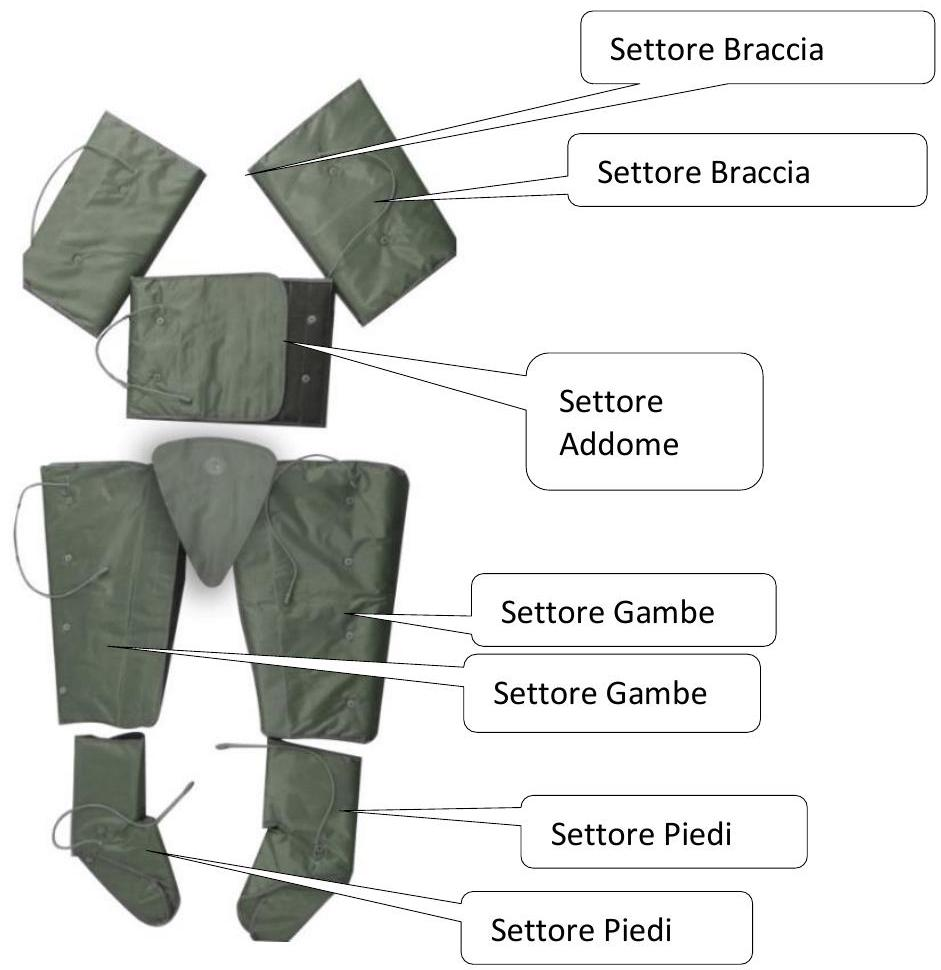
\includegraphics[max width=\textwidth, alt={}, center]{88087b73-f534-48df-a915-fe697c64a27c-23_970_941_125_208}

\subsubsection{Infrarossi (Apparecchio per il trattamento di calore parziale)}
\begin{itemize}
  \item Il sistema a infrarossi, con un effetto riscaldante, unito alla pressoterapia ed alla elettrostimolazione consente di tonificare e rassodare la massa muscolare, a scapito di quella adiposa.
  \item Riduce la quantità di grasso corporeo e soprattutto il grasso localizzato.
  \item Migliora il metabolismo, l'organismo diventa più efficiente nel consumare calorie e grasso. Migliora quindi l'aspetto estetico e la capacità dei muscoli di sfruttare l'adipe quale fonte energetica.
\end{itemize}

\subsubsection{Caratteristiche Generiche:}
\begin{itemize}
  \item canali già suddivisi tra tutte le zone del corpo con possibilità di scegliere la singola zona oppure il trattamento completo.
\end{itemize}

Mod. Rev.1.0 SLV 09-2020

\begin{itemize}
  \item Grazie alla gestione della temperatura su diversi livelli di intensità è possibile scegliere la funzionalità del trattamento: sudorazione, aumento del metabolismo, riattivazione del microciclo ed effetto rilassante.
\end{itemize}

\subsubsection{Elettrostimolatore}
\begin{itemize}
  \item La stimolazione muscolare ci aiuta a difendere la vitalità e la bellezza del nostro corpo stimolando e sviluppando la tonicità del nostro apparato muscolare.
  \item Il risultato è un aspetto più piacevole, una migliore forma fisica e una migliorata agilità nei movimenti.
  \item L' elettrostimolazione mirata ci permette di andare a risvegliare quei distretti muscolari non utilizzati (o utilizzato poco) da tempo che provocano lassità ad effetto cascata. Permette inoltre di combattere la cellulite e di agire sul sistema vascolare stimolando la circolazione linfatica.
  \item Questo apparato è stato progettato con attenzione secondo le ricerche di bionica umana, rottura del grasso, grasso dissolto, drenaggio linfatico, terapia magnetica e usa mezzi di alta tecnologia per massaggiare, questo fa sì che l'elettrostimolazione ed il massaggio ad aria diano un significativo risultato.
\end{itemize}

\subsubsection{Caratteristiche Generiche:}
\begin{itemize}
  \item canali
  \item Selezione delle uscite e regolazione dell'intensità di lavoro, personalizzazione del tipo di stimolazione.
  \item Programmi specifici per il trattamento della tonificazione.
\end{itemize}

\subsubsection{Dimagrimento}
\begin{itemize}
  \item I raggi infrarossi hanno un'azione diretta sulla struttura del grasso, rilasciando una grande energia termica, ne consegue un'accelerazione della circolazione sanguigna, stimolazione del metabolismo, accelerazione delle reazioni biochimiche, creazione del catabolismo nelle cellule del grasso, riduce le cellule del grasso
  \item Le sacche d'aria vengono gonfiate e sgonfiate regolarmente con pressione regolabile, questo dissocia e spacca le cellule di grasso.
\end{itemize}

\subsubsection{Abbellimento Corpo e Pelle}
\begin{itemize}
  \item La corrente elettrica stimola i terminali sensitivi nervosi della pelle, rendendola più bella ed elastica.
\end{itemize}

\subsubsection{Rilassamento}
\begin{itemize}
  \item La circolazione sanguigna sarà accelerata ed il muscolo diminuirà dopo che le micro correnti avranno lavorato nel corpo.
  \item L'energia termica generata dall'infrarosso diminuirà e rilasserà il muscolo.
\end{itemize}

\subsection{Principio di funzionamento}
Le seguenti indicazioni e metodi di trattamento sono da considerare solo di riferimento, i parametri e le procedure di funzionamento sono da valutare in funzione della clientela e vanno adattate ad ogni singolo soggetto. Consapevoli che in determinate operazioni di regolazione si possono raggiungere migliori risultati rispetto a condizioni e regolazioni più basse si deve considerare l'elevato rischio durante il trattamento con conseguenze sul cliente\\
Si consiglia pertanto l'utilizzo dell'apparecchiatura in sicurezza e sarebbe meglio consigliare alla clientela qualche trattamento in più che incorrere in rischi inutili.

\vspace{10pt}
Il tempo di applicazione varia in funzione del trattamento da effettuare ed è di norma variabile tra 15 e 60 minuti.

\vspace{10pt}
\noindent \textbf{Ad uso estetico il tempo massimo è di 30 minuti.}

\vspace{10pt}
È consigliabile procedere alla regolazione di intensità erogata, azionando lentamente i relativi comandi, avendo cura di operare con valori appena percettibili dal soggetto trattato.\\
Il soggetto trattato non dovrà avvertire fastidio, in caso contrario diminuire l'intensità di erogazione. Disattivando l'erogazione, l'intensità programmata si riporterà automaticamente a zero.

\section{Installazione e montaggio}
L'installazione ed il montaggio devono essere eseguiti da personale specializzato ed autorizzato. L’importatore o distributore declina ogni forma di responsabilità sia civile che penale per malfunzionamenti o difetti causati da cattiva installazione o mancata manutenzione periodica, essa va eseguita almeno una volta ogni dodici mesi, intervento a carico del cliente.

Seguire il manuale per l'installazione corretta ed installare in luogo idoneo.

Per la prima accensione ed installazione è fortemente consigliato l'intervento di un tecnico autorizzato.

\vspace{10pt}
\textbf{L'apparecchiatura deve essere usata solo ed esclusivamente presso locali e da personale specializzato ed autorizzato aventi i requisiti richiesti dalle normative vigenti. La formazione degli operatori è a carico dell'acquirente.\\
L'importatore, il distributore declinano ogni responsabilità civile e penale, amministrativa per un uso improprio della apparecchiatura}

\subsection{Installazione}
Collegare i tubi e i cavi prestando attenzione ai numeri delle uscite.

\begin{itemize}
	\item 
	\textbf{Fase 1}:
	Collegare i settori ai rispettivi tubi, seguendo l'ordine indicato.\\
	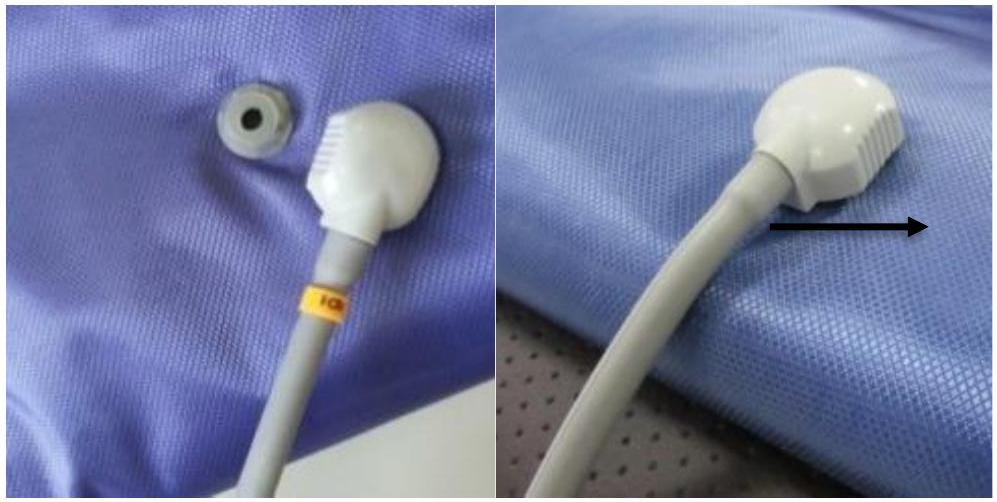
\includegraphics[max width=\textwidth, alt={}, center]{88087b73-f534-48df-a915-fe697c64a27c-26_502_997_1314_240}
%	
	\item 
	\textbf{Fase 2:}
	collegare i connettori nella parte posteriore alla macchina, seguendo attentamente i numeri riportati sulla macchina e sui connettori dei tubi.
%	
	\item 
	\textbf{Fase 3:}
	Una volta eseguite le procedure 1 e 2 collegare il cavo e procedere all’avvio premendo il tasto posteriore.
\end{itemize}

\subsection{Infrarosso}
\begin{figure}[h]
\begin{center}
  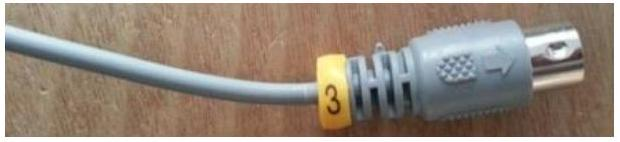
\includegraphics[alt={},max width=\textwidth]{88087b73-f534-48df-a915-fe697c64a27c-27_142_620_545_167}
\captionsetup{labelformat=empty}
\caption{Immagine 1}
\end{center}
\end{figure}

Connettori Infrarossi\\
1-2-3-4-5

Inserire i connettori (immagine 1) seguendo l'ordine indicato.

Il sistema a infrarossi, con un effetto riscaldante, unito alla pressoterapia ed alla elettrostimolazione consente di tonificare e rassodare la massa muscolare a scapito di quella adiposa.

Riduce la quantità di grasso corporeo e soprattutto il grasso localizzato.

Migliora il metabolismo, l'organismo diventa più efficiente nel consumare calorie e grasso. Migliora quindi l'aspetto estetico e la capacità dei muscoli di sfruttare l'adipe quale fonte energetica.

\subsection{Elettrostimolazione}
I cavi dell'elettrostimolazione si collegano con un connettore all'apparecchiatura, mentre nella parte opposta il cavo si divide in 2, nella parte con indicato il segnato con il simbolo "+" inserire l'elettrodo grande, mentre nell’altro cavo con il segno "- "mettere l'elettrodo piccolo.\\
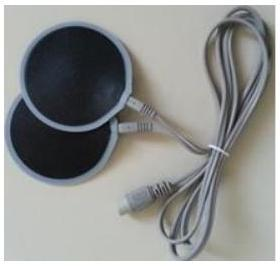
\includegraphics[max width=\textwidth, alt={}, center]{88087b73-f534-48df-a915-fe697c64a27c-28_266_280_177_247}\\
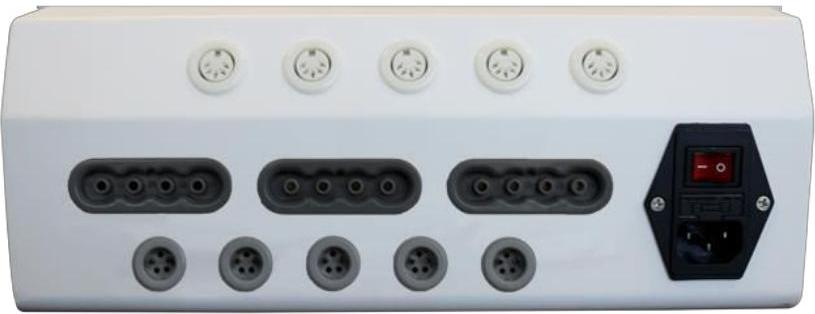
\includegraphics[max width=\textwidth, alt={}, center]{88087b73-f534-48df-a915-fe697c64a27c-28_314_815_174_560}

La stimolazione muscolare ci aiuta a difendere la vitalità e la bellezza del nostro corpo stimolando e sviluppando la tonicità del nostro apparato muscolare.

Il risultato è un aspetto più piacevole, una migliore forma fisica e una migliorata agilità nei movimenti.

L' elettrostimolazione mirata ci permette di andare a risvegliare quei distretti muscolari non utilizzati (o utilizzato poco) da tempo che provocano lassità ad effetto cascata. Permette inoltre di combattere la cellulite e di agire sul sistema vascolare stimolando la circolazione linfatica.

Questo apparato è stato progettato con attenzione secondo le ricerche di bionica umana, rottura del grasso, grasso dissolto, drenaggio linfatico, terapia magnetica e usa mezzi di alta tecnologia per massaggiare, questo fa sì che l'elettrostimolazione ed il massaggio ad aria diano un significante effetto.

\subsection{Installazione ed accensione}
\begin{enumerate}
  \item Collegare il cavo di alimentazione.
  \item Accendere l'apparecchiatura premendo il tasto posteriore.
  \item Collegare rispettivamente le uscite delle sacche d'aria.
\end{enumerate}

\subsection{Massaggio ad Aria}
I cuscinetti vengono applicati sulle parti da trattare, per effettuare un massaggio con pressione alternata, sequenziale. Rispettare i tempi, le pressioni e le frequenze di trattamento secondo le

Pag. 27 Mod. Rev.1.0 SLV 09-2020\\
indicazioni fornite in fase di installazione.\\
Non usare in soggetti con fragilità capillare, ipertensione arteriosa o cardiopatie.

\vspace{10pt}
\noindent \textbf{AVVERTENZE:}\\
Si raccomandano le idonee sterilizzazioni e/o disinfezioni di tutte le parti che vanno a contatto col soggetto da trattare.

\section{Utilizzo}
\noindent \faExclamationTriangle \textbf{CAUTION}:
\\
Tutte le persone che utilizzeranno la macchina devono studiare questo manuale con molta attenzione ed in seguito, prendere le misure di sicurezza necessarie, prima di iniziare una qualsiasi delle procedure. L'utilizzo errato di tale apparecchiatura potrebbe causare gravi danni alla salute del cliente.

\subsection{Operatività presso massaggio}

\begin{figure}[H]
\begin{center}
%\captionsetup{labelformat=empty}
  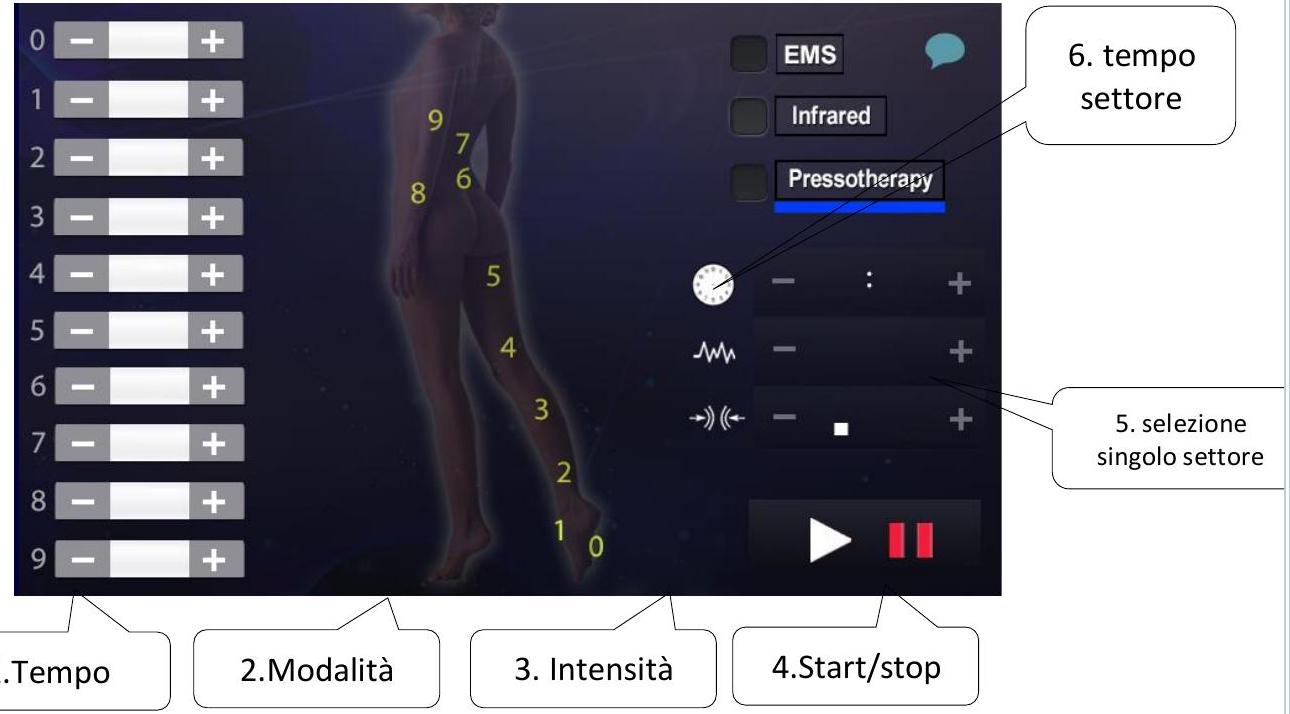
\includegraphics[alt={},max width=\textwidth]{88087b73-f534-48df-a915-fe697c64a27c-29_714_1290_817_117}
\end{center}
\end{figure}

\begin{enumerate}
  \item Premendo i tasti "+" "-" sì regola il tempo totale del trattamento, il massimo ad uso estetico è di 30 Minuti.
  \item Premendo i tasti "$\blacktriangledown$" "$\blacktriangle$" sì sceglie le modalità che sono 4: (A, B, C, D)
\end{enumerate}

\begin{itemize}
	\item \textbf{Programma A - MASSAGGIO PERISTALTICO-LINFODRENAGGIO MANUALE}
	Parte dai piedi e ogni settore viene gonfiato singolarmente, una volta arrivato alle braccia gonfia tutti i gonfianti in contemporanea. La pressione viene esercitata da una sola camera alla volta in modo settoriale (i settori si gonfiano uno alla volta: si gonfia il primo e poi quando si gonfia il secondo si sgonfia il primo e così via). Queste azioni vengono comunque svolte solo sull'arto a cui è applicato il terminale e non su tutte le zone del cliente, come previsto dai metodi di linfodrenaggio classico. Questa simulazione di linfodrenaggio manuale è molto utile per combattere problemi di ritenzione idrica e gonfiori. I fluidi vengono spinti sia nella direzione corretta fisiologica (distoprossimale) che in quella retrograda.
%	
	\item \textbf{Programma B - MASSAGGIO PROFONDO-LINFODRENAGGIO}
	Le camere vengono progressivamente riempite d'aria dall'estremità distale verso quella prossimale e l'aria entra nella camera successiva solo quando in quella precedente ha raggiunto il livello preimpostato per il trattamento e tutte le camere restano gonfie finché anche nell'ultima si è raggiunta la pressione precedentemente regolata. Grazie a questo programma si ottiene un vero e proprio "svuotamento": la spinta omogenea e continua effettua in maniera ottimale lo svuotamento dell'arto da fluidi che ristagnano.
	\\
	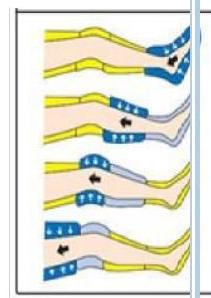
\includegraphics[max width=\textwidth, alt={}, center]{88087b73-f534-48df-a915-fe697c64a27c-30_298_211_537_1211}
%	
	\item \textbf{Programma C - SISTEMA SEQUENZIALE (MASSAGGIO D'URTO)}
	Parte dal basso e arriva fino alle braccia. Questo programma comporta che tutti i settori che compongono il gambale o il bracciale si gonfiano uno dopo l'altro a partire da quello più periferico, piede o mano, sino all'ultimo e solo quando quest'ultimo ha raggiunto la pressione desiderata, i sgonfiano tutti insieme. La pressione di gonfiaggio viene, quindi, esercitata su tutte parti montate. Questo tipo di programma rappresenta la possibilità di utilizzare al meglio questa apparecchiatura come trattamento d'urto contro la cellulite e la ritenzione idrica più importante.
	\\
	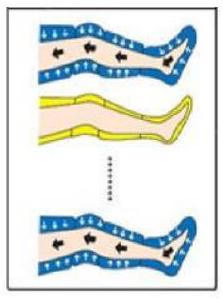
\includegraphics[max width=\textwidth, alt={}, center]{88087b73-f534-48df-a915-fe697c64a27c-31_299_223_276_1035}
%	
	\item \textbf{Programma D - MASSAGGIO MISTO}
	Con il programma D si gonfierà in 3 linee contemporaneamente, sotto riportata la tabella.
\end{itemize}

\begin{center}
\begin{tabular}{|l|l|l|l|l|l|}
\hline
Fase 1 & Fase 2 & Fase 3 & Fase 4 & Fase 5 & Fase 6 \\
\hline
0 & 1 & 2 & 3 & 4 & 5 \\
\hline
6 & 7 & 6 & 7 & 6 & 7 \\
\hline
9 & 8 & 9 & 8 & 9 & 8 \\
\hline
\end{tabular}
\end{center}

Questo tipo di trattamento è quello più rilassante, ma proprio per questo non è indicata per combattere la ritenzione idrica e la cellulite. Il massaggio misto può essere utilizzato per procedere con un semplice massaggio rilassante.\\
3. Premendo i tasti "$\blacktriangledown$" "$\blacktriangle$" si regola l'intensità che varia da 1 a 3 .\\
4. Start/stop\\
5. Premendo i tasti "$\blacktriangledown$" "$\blacktriangle$" si regola la durata di gonfiaggio dei singoli settori.\\
6. Premendo il quadrato indicato, il settore non sarà gonfiato, e all'interno del quadrato uscirà il simbolo: "- - "

\subsection{Operatività infrarosso}

\begin{figure}[H]
\begin{center}
%\captionsetup{labelformat=empty}
  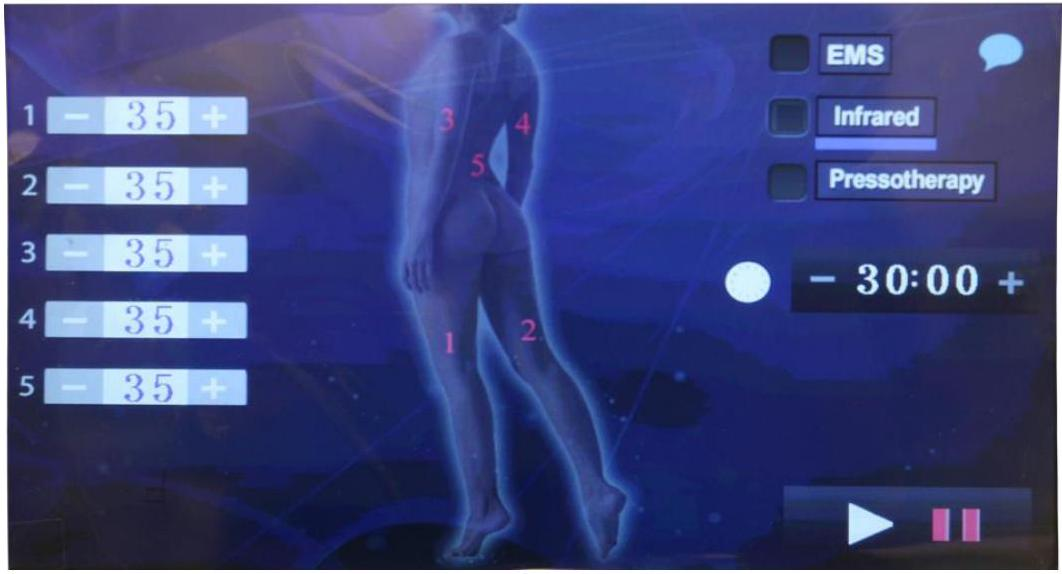
\includegraphics[alt={},max width=\textwidth]{88087b73-f534-48df-a915-fe697c64a27c-32_574_1062_465_242}
\end{center}
\end{figure}

L'infrarosso ha dei valori che vanno da 35 a Max 65.\\
Per deselezionare l'infrarosso premere sul valore numerico Il valore da scegliere per l'infrarosso va in base alla sensibilità del cliente. Il sistema ad infrarossi, con un effetto riscaldante, unito alla pressoterapia ed alla elettrostimolazione (opzionale) consente di tonificare e rassodare la massa muscolare, a scapito di quella adiposa. Riduce la quantità di grasso corporeo e soprattutto il grasso localizzato. Migliora il metabolismo, l'organismo diventa più efficiente nel consumare calorie e grasso. Migliora quindi l'aspetto estetico e la capacità dei muscoli di sfruttare l'adipe quale fonte energetica.

\subsection{Operatività E.M.S (Elettrostimolazione)}
\begin{center}
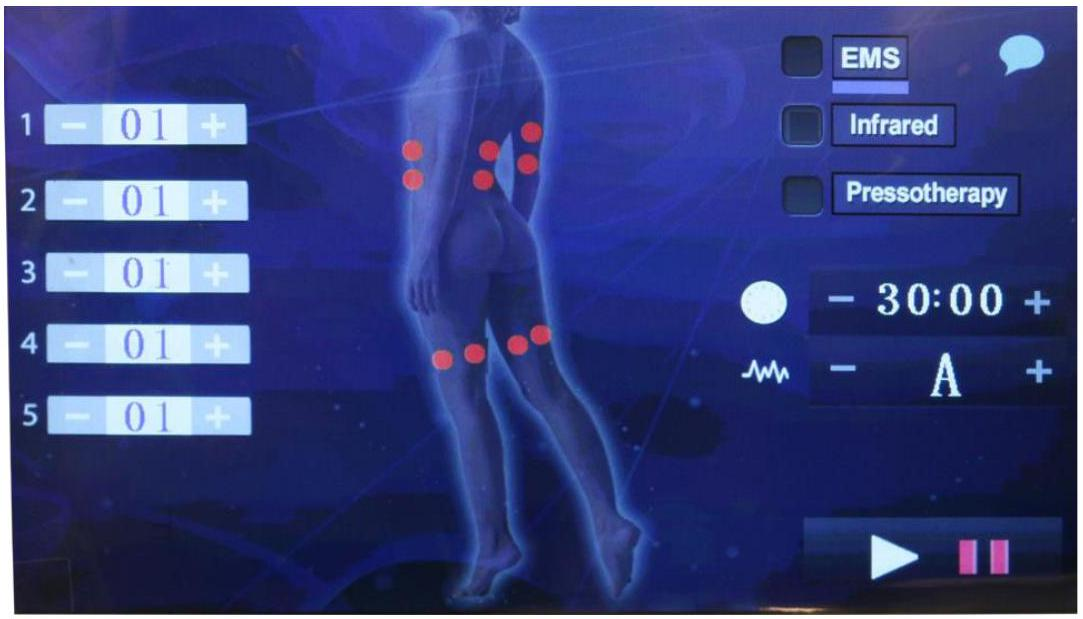
\includegraphics[max width=\textwidth, alt={}]{88087b73-f534-48df-a915-fe697c64a27c-33_619_1083_180_168}
\end{center}

La stimolazione muscolare ci aiuta a difendere la vitalità e la bellezza del nostro corpo stimolando e sviluppando la tonicità del nostro apparato muscolare.

Il risultato è un aspetto più piacevole, una migliore forma fisica e una migliorata agilità nei movimenti.

L' elettrostimolazione mirata ci permette di andare a risvegliare quei distretti muscolari non utilizzati (o utilizzato poco) da tempo che provocano lassità ad effetto cascata. Permette inoltre di combattere la cellulite riducendo le cellule di grasso. Permette, d'agire sul sistema vascolare stimolando la circolazione linfatica.

Tonifica e rassoda la muscolatura del corpo, facilita ed incrementa l'eliminazione delle tossine, stimola il drenaggio linfatico, agisce contro gli inestetismi della cellulite e contrasta la ritenzione idrica. Ulteriore effetto benefico per la persona è la piacevole sensazione di relax e benessere ricevuta durante il trattamento che persiste durante il proseguimento dell'attività quotidiana.

Il tempo di applicazione varia in funzione del trattamento da effettuare ed è, di norma variabile tra 15 e 60 minuti. È consigliabile procedere alla regolazione di intensità di corrente erogata,\\
azionando lentamente i relativi comandi, avendo cura di operare con valori appena percettibili dal soggetto trattato.\\
\textbf{Il soggetto trattato non dovrà avvertire fastidio, in caso contrario diminuire l'intensità di erogazione.}

\vspace{10pt}
\textbf{Disattivando l'erogazione, l'intensità programmata si riporterà automaticamente a zero:}

\vspace{10pt}
\textbf{4 programmi:}
\begin{itemize}
	\item 
	\textbf{A}: Bassa frequenza e dissolvenza adipe (inestetismo superficiale)\\
	Ruolo: II segnale agisce direttamente sulle cellule adipose, espandendole e rendendole di più semplice decomposizione. Questo aiuta il processo di espulsione dell'adipe.\\
	Scopo: È adatto ad ogni processo di perdita di peso, specialmente le adiposità localizzate.
%	
	\item 
	\textbf{B}: Cellulite profonda\\
	Ruolo: Il segnale stimola i tessuti muscolari a produrre contratture atte a tonificare il muscolo e che agendo sull'adipe sottostante, stimolano la produzione di creatina muscolare, la quale decompone e scioglie il grasso.\\
	Scopo: Adipe profondo
%	
	\item 
	\textbf{\textbf{C}}: Esercizio muscolare (potenziamento e rafforzamento)\\
	Ruolo: L'intensità delle pulsazioni e della frequenza migliora la stimolazione delle fibre muscolari e scioglie l'adipe profondo.
%	
	\item 
	\textbf{D}: Perdita di peso continuativa (brucia grassi detox)\\
	Ruolo: II segnale penetra in profondità nei muscoli e aumentando la circolazione linfatica, elimina le tossine e gli acidi grassi idrogenati. Scopo: viene usato in casi di disordine della circolazione linfatica, obesità dovuta a liquidi trattenuti e trattamenti detox.
\end{itemize}





'\begin{figure}[H]
\begin{center}
\captionsetup{labelformat=empty}
\caption{Posizionamento elettrodi}
  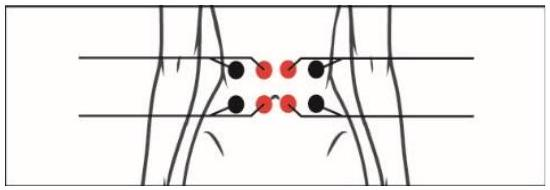
\includegraphics[alt={},max width=\textwidth]{88087b73-f534-48df-a915-fe697c64a27c-35_190_550_342_167}
\end{center}
\end{figure}

\begin{center}
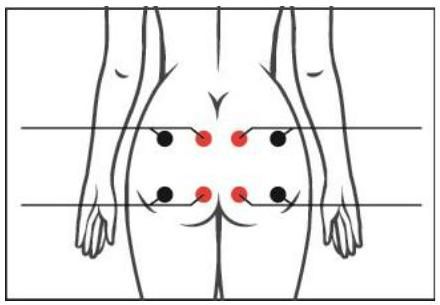
\includegraphics[max width=\textwidth, alt={}]{88087b73-f534-48df-a915-fe697c64a27c-35_305_440_340_778}
\end{center}

\noindent \faExclamationTriangle \textbf{CAUTION}:
\\
Tutte le persone che utilizzeranno la macchina devono studiare questo manuale con molta attenzione ed in seguito, prendere le misure di sicurezza necessarie, prima di iniziare una qualsiasi delle procedure. L'utilizzo errato di tale apparecchiatura potrebbe causare danni alla salute del cliente.

\subsection{Indicazioni}
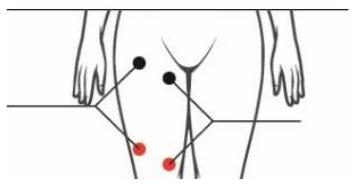
\includegraphics[max width=\textwidth, alt={}, center]{88087b73-f534-48df-a915-fe697c64a27c-35_187_355_1017_138}\\
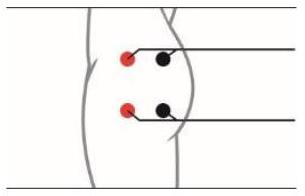
\includegraphics[max width=\textwidth, alt={}, center]{88087b73-f534-48df-a915-fe697c64a27c-35_196_305_1020_558}\\
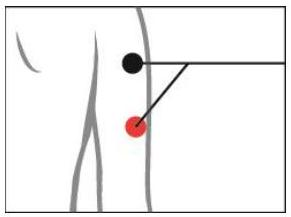
\includegraphics[max width=\textwidth, alt={}, center]{88087b73-f534-48df-a915-fe697c64a27c-35_217_291_1020_934}

Attenzione le indicazioni riportate sono puramente indicative, esse vanno valutate in funzione del trattamento e della persona da trattare qualsiasi impostazione o indicazione va considerata puramente indicativa, l'operatore deve valutare di volta in volta ed in funzione del soggetto da trattare tutti i parametri e valutare le controindicazioni che si possono incontrare con ogni singolo soggetto.

Sono disponibili presso la nostra azienda corsi di formazione ed informazione sul corretto uso dell'attrezzatura, tutti gli utilizzatori devono e si devono, prima dell'utilizzo dell'apparecchiatura, informare sui seguenti argomenti:

\begin{itemize}
  \item Uso dell'apparecchiatura con l'ausilio di un formatore e del manuale d'uso,
  \item Principio di funzionamento,
  \item Uso specifico del modello in dotazione nell'istituto od ambulatorio,
  \item Applicazioni e avvertenze sull'uso dell'apparecchiatura,
  \item Effetti collaterali,
  \item Informazione presso altri istituti e/o conoscenze sul corretto uso dell'apparecchiatura,
  \item Studio di tutte le avvertenze,
  \item Informazione sui sistemi di sicurezza da adottare,
  \item Cosa si deve fare in caso di anomalia tecnica o di lesioni procurate,
\end{itemize}

\textbf{L'apparecchiatura è adatta a:}
\begin{itemize}
  \item Inestetismi provocati da cellulite,
  \item Ritenzione idrica,
  \item Sovrappeso,
\end{itemize}

Tonificazione dei tessuti,

\subsection{Controindicazioni}
\begin{itemize}
  \item Persone con emofilia,
  \item Persone con pacemaker,
  \item Persone con malattie cardiovascolari,
  \item Persone con allergie alla pelle,
  \item Persone con febbre ,
  \item Donne in gravidanza,
  \item Portatori di Handicap,
  \item Persone di Minore età,
  \item Epilessia,
  \item Dispositivi di incontinenza, pompa insulina,
  \item Insufficienza cardiaca,
  \item Lesioni cutanee: erisipela, micosi, piodermiti,
  \item Linfangiti,
  \item Tromboflebiti,
  \item Flebite
  \item Tubercolosi,
  \item Insufficienza arteriosa periferica grave,
  \item Plessopatia e neuropatia,
  \item Gravi infezioni
  \item Tumori
  \item Ipertensione
  \item Ipotensione
  \item Asma
  \item Problemi renale
  \item \textbf{In presenza di qualsiasi altra condizione che secondo il medico curante potrebbe rendere insicuro il trattamento}
  \item \textbf{In caso di dubbi far consultare il proprio medico curante}
\end{itemize}

\subsubsection{Non Trattare:}

\vspace{10pt}
\textbf{Portatori di impianti attivi come:}
\begin{itemize}
  \item Pacemaker,
  \item Pompa insulina,
  \item Portatori di protesi articolari metalliche,
  \item Soggetti con processi flogistici in atto,
  \item Soggetti con lesioni cutanee,
  \item Soggetti con neoplasie,
  \item Donne in stato di gravidanza,
  \item Non trattare soggetti con pelle sensibile, eventualmente limitarsi a potenze di erogazione molto basse,
  \item Presenza di neoplasie nella zona scelta per il trattamento,
  \item Presenza di infezioni, o di dermatiti, nella zona da trattare,
  \item Chi soffre di insufficienza arteriosa o cardiaca,
  \item Chi soffre di vene varicose,
  \item Chi soffre di tromboflebiti, oppure di trombosi venosa profonda,
  \item Chi abbia subito da poco interventi per innesto di pelle,
  \item Applicare solo su pelle integra.
\end{itemize}

In caso di dubbi far consultare il proprio medico curante

\subsection{Effetti Collaterali}
Una delle conseguenze secondarie è la flogosi cronica, ossia una infiammazione non passeggera nella zona trattata. Si pensi ancora alla possibilità di un indurimento cutaneo, provocato appunto dalla\\
accresciuta pressione esercitata sulla area del corpo interessata dalla pressoterapia. Possibile è anche che i capillari presenti nella zona interessata dal trattamento possano rompersi, a causa dell'eccessiva pressione esercitata dal macchinario.

Lieve rossore, tepore per i modelli dell'apparecchiatura con elettrostimolatore e infrarosso.

\section{Manutenzione:}
\noindent \faExclamationTriangle \textbf{CAUTION}:
\\
Tutte le persone che utilizzeranno la macchina devono studiare questo manuale con molta attenzione ed in seguito, prendere le misure di sicurezza necessarie, prima di iniziare una qualsiasi delle procedure. L'utilizzo errato di tale apparecchiatura potrebbe causare gravi danni alla salute del cliente.

\vspace{5pt}
\noindent \textbf{Manutenzione e risoluzione dei problemi}

\vspace{5pt}
Il sistema può funzionare correttamente solo se tutte le seguenti condizioni sono soddisfatte:

\begin{itemize}
  \item Il personale ha soddisfatto tutte le norme di sicurezza
  \item Il personale ha letto il manuale d'uso
  \item L'apparecchio è ben collegato con la presa di alimentazione.
  \item Interruttore posto nella parte posteriore in posizione ON.
\end{itemize}

\noindent \faExclamationTriangle \textbf{CAUTION}:
\\
L'apparecchiatura deve essere usata solo ed esclusivamente presso locali e da personale specializzato ed autorizzato aventi i requisiti richiesti dalle normative vigenti. La formazione degli operatori è a carico dell'acquirente.

\subsection{Manutenzione e pulizia}
\noindent \faExclamationTriangle \textbf{CAUTION}:
\\
Qualsiasi operazione di pulizia deve essere eseguita con apparecchiatura scollegata dalla rete elettrica

\begin{itemize}
  \item Una corretta manutenzione è necessaria per garantire che il sistema funzioni perfettamente,
  \item Si raccomandano le idonee sterilizzazioni e/o disinfezioni di tutte le parti che saranno a contatto con il soggetto da trattare,
  \item In caso di anomalie o dubbi contattare il servizio di assistenza,
  \item La manutenzione e la sostituzione di eventuali ricambi deve essere fatta solo da personale qualificato ed autorizzato,
  \item La mancata manutenzione periodica e il non utilizzo di ricambi originali può far perdere i diritti di garanzia, ma soprattutto si può mettere l'apparecchiatura in condizioni pericolose per la clientela,
  \item Qualsiasi tipo di manutenzione o di pulizia deve essere effettuata con alimentazione della corrente scollegata,
  \item Nel caso l'apparecchiatura non dovesse essere usata per parecchio tempo (es. Ferie) provvedere alla sua copertura per evitare polveri, agenti inquinanti ed umidità e scollegarla completamente dalla rete elettrica,
  \item In caso di manutenzione scollegare l'apparecchiatura dalla rete elettrica,
  \item Non togliere mai le coperture di protezione se non scollegato dalla rete elettrica,
  \item Verificare che il luogo di installazione dell'apparecchiatura sia perfettamente integro, pulito e con bassa percentuale di umidità, privo di polvere, questi elementi possono influenzare il corretto funzionamento, diminuirne l'efficacia ed influenzarne il perfetto funzionamento,
  \item Evitare che l'apparecchiatura sia in una posizione che può essere colpita direttamente dai raggi solari,
  \item \textbf{Al termine di ogni trattamento pulire e disinfettare il kit con appositi prodotti e lasciare raffreddare le dotazioni aperte, in modo da evitare problemi di surriscaldamento ai circuiti interni. L'eventuale malfunzionamento derivante dal non rispetto di tale avvertenza, non verrà riconosciuto dal distributore/costruttore come danno in garanzia.}
\end{itemize}

\subsection{Manutenzione}
\begin{itemize}
  \item Controllare regolarmente le prese d'aria ai lati, mantenerle pulite da polveri e posizionare l'apparecchiatura almeno tra gli\\
$80 / 100 \mathrm{~cm}$ da qualsiasi ostacolo, tende, muri ecc. non appoggiarla su teli o coperte e fare in modo che l'apparecchiatura usufruisca di maggior aria possibile.
\end{itemize}

\subsection{Guida alla risoluzione dei problemi}
Solo il personale qualificato ed autorizzato può aprire l'apparecchiatura, prima di procedere a tale operazione scollegare dalla presa di rete.

\subsubsection{La Pressoterapia non si accende}
Verificare che le seguenti voci siano state completate.

\begin{itemize}
  \item Il cavo di alimentazione sia saldamente e completamente inserito nella presa di alimentazione sul pannello posteriore e in una presa di corrente funzionante,
  \item L'interruttore principale sul pannello posteriore è su ON.
  \item Controllare o sostituire il fusibile. Scollegare l'apparecchiatura dalla rete elettrica e con apposito cacciavite, procedere alla sostituzione con fusibile appropriato indicato in etichetta,
\end{itemize}

Se il problema persiste, contattare l'Assistenza clienti.

\section{Allegati al manuale}

\subsection{Scheda Tecnica}

\begin{figure}[H]
	\centering
	\includegraphics[width=\linewidth]{"images/Schermata del 2026-03-16 16-10-08"}
%	\caption{}
	\label{fig:schermata-del-2026-03-16-16-10-08}
\end{figure}


%\begin{table}[H]
%	\centering
%\begin{tabularx}{\linewidth}{|X|X|X|X|X|}
%\hline
%\multicolumn{5}{|l|}{SPECIFICHE TECNICHE} \\
%\hline
%Apparecchiatura: & \multicolumn{4}{|l|}{Presso Massaggio} \\
%\hline
%Modello: (IN BASE AL MODELLO SCELTO) & 2 IN1 & Presso massaggio base &  &  \\
%\hline
%Display: & \multicolumn{4}{|l|}{Color LCD Touch Screen 6,7 Pollici} \\
%\hline
%Numero Settori: & 10 & 4 gambe & 2 addome & 2 braccia \\
%\hline
%Uscite: & \multicolumn{4}{|l|}{12 aria 5 infrarosso} \\
%\hline
%Peso marsupio completo: & \multicolumn{4}{|l|}{8 Kg} \\
%\hline
%Programmi Presso: & \multicolumn{4}{|l|}{4 con potenza regolabile} \\
%\hline
%Programmi Infrarosso: & \multicolumn{4}{|l|}{potenza regolabile} \\
%\hline
%Programmi Elettrostimolazione: & \multicolumn{4}{|l|}{potenza regolabile} \\
%\hline
%Alimentazione: & \multicolumn{4}{|l|}{AC $230-240 \mathrm{~V} 50 / 60 \mathrm{~Hz}$} \\
%\hline
%Assorbimenti: & \multicolumn{4}{|l|}{Standby $0,1 \mathrm{~A} / 0,5 \mathrm{~W}-\mathrm{Max} 0,20 \mathrm{~A} / 30 \mathrm{~W}$} \\
%\hline
%Peso Netto: & \multicolumn{4}{|l|}{$\pm 6 \mathrm{Kg}$} \\
%\hline
%Dimensione Fisica: & \multicolumn{4}{|l|}{$34 \times 36 \times 20 \mathrm{~cm}$ (montato)} \\
%\hline
%Temperatura Trasporto e Stoccaggio: & \multicolumn{4}{|l|}{$\min 10^{\circ} \mathrm{C}-\operatorname{Max} 40^{\circ} \mathrm{C}$} \\
%\hline
%Temperatura Ambiente: & \multicolumn{4}{|l|}{$\min 10^{\circ} \mathrm{C}-\operatorname{Max} 30^{\circ} \mathrm{C}$} \\
%\hline
%\end{tabularx}
%\end{table}

L'apparecchiatura deve essere usata solo ed esclusivamente presso locali e da personale specializzati ed autorizzati aventi i requisiti richiesti. La formazione degli operatori è a carico dell'acquirente. Le caratteristiche tecniche possono subire variazioni, le immagini sono puramente indicative. L'importatore e il distributore declinano ogni responsabilità civile, penale ed amministrativa per un uso improprio della apparecchiatura.\\
È responsabilità civile e penale di chi detiene o utilizza l'apparecchiatura seguire le indicazioni e le normative vigenti a livello nazionale o regionale ove l'apparecchiatura viene installata. È buona norma da parte dell'utilizzatore o acquirente verificare che l'apparecchiatura rientri nelle normative in vigore nel momento dell'acquisto. All'interno degli ambienti di utilizzo devono essere osservate tutte le normative che regolamentano la sicurezza sul lavoro del personale e le normative che regolamentano la sicurezza degli ambienti.\\
Attualmente il D.lgs. 206 del 15 ottobre 2015 relativo agli apparecchi elettromeccanici utilizzati per I'attività di estetista, impone delle nuove regole, tra cui l'obbligo per alcune apparecchiature di un corso % manca un pezzo nell'originale?

\newpage

\section{CONSENSO INFORMATO - Trattamento estetico "DRENALINPHA+"}
\subsection{DATI CLIENTE}
\noindent Nome e Cognome: $\_\_\_\_$\\
Data di nascita: $\_\_\_\_$\\
Telefono: $\_\_\_\_$

\subsection{DATI OPERATORE / CENTRO}
\noindent Nome centro: $\_\_\_\_$\\
Operatore: $\_\_\_\_$

\subsection{DESCRIZIONE DEL TRATTAMENTO}
Il trattamento Drenalinpha+ è un protocollo estetico finalizzato a stimolare il sistema linfatico, favorire il drenaggio dei liquidi, migliorare la circolazione superficiale e ridurre la sensazione di gonfiore e pesantezza.

\subsection{POSSIBILI EFFETTI}
Lieve arrossamento temporaneo, sensazione di calore, lieve sensibilità nella zona trattata.

\subsection{CONTROINDICAZIONI}
Gravidanza, patologie cardiache o circolatorie importanti, infezioni o infiammazioni in atto, patologie oncologiche in corso, problematiche linfatiche gravi non diagnosticate, uso di farmaci anticoagulanti.

\subsection{DICHIARAZIONI DEL CLIENTE}
Dichiaro di aver ricevuto spiegazioni chiare, di essere a conoscenza che si tratta di trattamento estetico e non medico, e di autorizzare l'esecuzione del trattamento.

\subsection{PRIVACY}
I dati saranno trattati nel rispetto del Regolamento UE 2016/679 (GDPR).\\
Firma Cliente: $\_\_\_\_$\\
Firma Operatore: $\_\_\_\_$\\
Data: $\_\_\_\_$ 1 $\_\_\_\_$ $/$ $\_\_\_\_$

% --- INIZIO INFORMATIVA PRIVACY ---
\newpage

\section{INFORMATIVA PRIVACY}
\begin{center}
	(ai sensi dell'art. 13 del Regolamento UE 2016/679)
\end{center}

La presente informativa è resa ai sensi del Regolamento Generale sulla Protezione dei Dati (GDPR) e riguarda il trattamento dei dati personali dei clienti che si sottopongono a trattamenti e tecnologie estetiche.

\subsection*{Titolare del trattamento}

Il Titolare del trattamento è:

\begin{itemize}
	\item Denominazione centro estetico: \underline{\hspace{5cm}}
	\item Sede legale: \underline{\hspace{7cm}}
	\item P. IVA / C.F.: \underline{\hspace{6cm}}
	\item Contatti (telefono/email): \underline{\hspace{5cm}}
\end{itemize}

\subsection*{Tipologia di dati trattati}

Il Titolare può raccogliere e trattare le seguenti categorie di dati:

\begin{itemize}
	\item Dati anagrafici (nome, cognome, data di nascita)
	\item Dati di contatto (telefono, e-mail)
	\item Dati fiscali per eventuale fatturazione
	\item Dati particolari relativi allo stato di salute (allergie, patologie, gravidanza, terapie in corso) necessari per valutare l'idoneità ai trattamenti estetici
	\item Eventuali immagini fotografiche prima/dopo trattamento (previo consenso specifico)
\end{itemize}

\subsection*{Finalità del trattamento}

I dati personali sono trattati per le seguenti finalità:

\begin{enumerate}
	\item Esecuzione di trattamenti estetici e utilizzo di tecnologie professionali (laser, radiofrequenza, ultrasuoni, pressoterapia, ecc.)
	\item Valutazione dell'idoneità al trattamento
	\item Adempimenti amministrativi, contabili e fiscali
	\item Gestione degli appuntamenti
	\item Eventuale invio di comunicazioni promozionali (solo previo consenso separato)
	\item Eventuale utilizzo di immagini per finalità informative o promozionali (solo previo consenso separato)
\end{enumerate}

\subsection*{Base giuridica del trattamento}

Il trattamento dei dati si fonda su:

\begin{itemize}
	\item Esecuzione del contratto/prestazione richiesta
	\item Adempimento di obblighi di legge
	\item Consenso esplicito dell'interessato per il trattamento di dati particolari (sanitari)
	\item Consenso separato per marketing e utilizzo immagini
\end{itemize}

\subsection*{Modalità di trattamento}

Il trattamento dei dati avviene mediante strumenti cartacei e/o informatici, nel rispetto dei principi di correttezza, liceità, trasparenza e tutela della riservatezza.

Sono adottate adeguate misure di sicurezza per prevenire accessi non autorizzati, perdita o diffusione dei dati.

\subsection*{Conservazione dei dati}

I dati personali saranno conservati:

\begin{itemize}
	\item Per il tempo necessario all'erogazione del servizio
	\item Per il periodo previsto dalla normativa fiscale e civilistica
	\item Fino a revoca del consenso per finalità di marketing o utilizzo immagini
\end{itemize}

\subsection*{Comunicazione dei dati}

I dati potranno essere comunicati a:

\begin{itemize}
	\item Consulenti fiscali e amministrativi
	\item Software gestionali utilizzati per la gestione clienti
	\item Autorità competenti, ove previsto dalla legge
\end{itemize}

I dati non saranno diffusi senza consenso.

\subsection*{Diritti dell'interessato}

L'interessato può esercitare in qualsiasi momento i seguenti diritti:

\begin{itemize}
	\item Accesso ai propri dati
	\item Rettifica o aggiornamento
	\item Cancellazione (diritto all'oblio)
	\item Limitazione del trattamento
	\item Opposizione al trattamento
	\item Revoca del consenso
	\item Reclamo all'Autorità Garante per la Protezione dei Dati Personali
\end{itemize}

Le richieste possono essere inviate ai recapiti del Titolare sopra indicati.

\subsection*{Natura del conferimento dei dati}

Il conferimento dei dati è necessario per l'erogazione dei trattamenti estetici.
Il mancato conferimento può comportare l'impossibilità di eseguire il servizio.

\subsection*{CONSENSO}

Il/La sottoscritto/a dichiara di aver ricevuto e compreso la presente informativa.

\vspace{0.8cm}

Data: \underline{\hspace{5cm}} 

\vspace{15pt}
Firma: \underline{\hspace{6cm}}

\vspace{1cm}

$\square$ Acconsento al trattamento dei dati particolari (sanitari)

\vspace{0.3cm}
$\square$ Acconsento all'utilizzo delle immagini per finalità promozionali

\vspace{0.3cm}
$\square$ Acconsento a ricevere comunicazioni promozionali

% --- FINE INFORMATIVA PRIVACY ---

\newpage


\begin{figure}[H]
	\centering
	\includegraphics[width=0.7\paperwidth,height=\paperheight, keepaspectratio]{"../cose da aggiungere/privacy_conformita/dichiarazione_conformita"}
\end{figure}



\end{document}